\documentclass{article}

\usepackage[utf8]{inputenc}
\usepackage[T1]{fontenc}

\usepackage[authoryear,round]{natbib}
\bibliographystyle{abbrvnat}

\usepackage[french]{babel}

\usepackage[a4paper, margin=2.54cm]{geometry}
\usepackage{graphicx}
\usepackage{multirow}
\usepackage{tabularx}
\usepackage[dvipsnames]{xcolor}
\usepackage[autolanguage]{numprint}

\usepackage[colorlinks=true,citecolor=teal,linkcolor=Periwinkle,urlcolor=Periwinkle]{hyperref}

\newcommand{\subsubsubsection}[1]{\paragraph{#1}\par\noindent\bigskip}
\newcommand{\method}[1]{\hspace{1in}\texttt{#1}\bigskip}

\renewcommand\labelitemii{$\bullet$}

\linespread{1.2}

\begin{document}

% Page de titre
{
    \begin{titlepage}
        \begin{center}
            \vspace*{2.54cm}

            \Large \textbf{Extension de recalage pour 3D~Slicer}

            \vspace{2.54cm}

            \large \textbf{Wissam~Boussella, Iantsa~Provost, Bastien~Soucasse \\ et~Tony~Wolff}

            \vfill

            Un devoir présenté dans le cadre du \\ projet de fin d'études.

            \vspace{2.54cm}

            
\includegraphics[width=.5\textwidth]{images/ub.jpg}

            Master informatique pour l'image et le son \\ Université de Bordeaux, France
        \end{center}
    \end{titlepage}
    \newpage
    \setcounter{page}{2}
}

% Table des matières
{
    \hypersetup{linkcolor=black}
    \tableofcontents
    \newpage
}

% Introduction
{
    \section{Introduction}
    \label{sec:introduction}

    Dans le contexte de notre projet de fin d'études, nous avons développé un outil de recalage d'images 3D dans le domaine médical. Il s'agit d'une extension pour le logiciel de traitements d'images 3D médicales 3D~Slicer.

    \bigskip

    La volonté du client était d'agréger en une même interface au sein de 3D~Slicer des algorithmes de prétraitements (en particulier sélection de ROI, rognage, et rééchantillonnage), de recalage, et de calcul de carte de différence, tout en donnant la possibilité d'ajouter le plus simplement possible de nouveaux algorithmes a posteriori. Dans le cadre d'une extension intégrée à 3D~Slicer, le client avait également la volonté de pouvoir visualiser les images (avant et après traitement) et les cartes de différences en parallèle.

    \bigskip

    Le projet a donc été développé en Python de sorte de correspondre à 3D~Slicer. Différentes bibliothèques sont intégrées à 3D~Slicer et sont à utiliser dans ce projet. Le client nous a informé vouloir se contenter d'algorithmes de deux bibliothèques dont il connaît l'utilisation~: ITK et Elastix.

    \bigskip

    Le projet a été conçu et mené en suivant la méthode agile SCRUM, c'est-à-dire que le projet a été développé sur différents \textit{sprints} (succession de tâches à terminer avant la prochaine itération) et axé sur les tests avant l'implémentation~: c'est le Test-Driven Development (TDD).

    \bigskip

    Ce rapport synthétise notre expérience sur le projet. Il décrit tout d'abord les travaux connexes au traitement et recalage d'images 3D médicales. Nous explicitons ensuite la conception du projet en détaillant les User Stories qui représentent très précisément les différents besoins du client, qui nous ont aidé à garder une ligne directrice durant le développement du projet. Les tests sont ensuite décrits dans ce rapport, avant de détailler concrètement l'implémentation. Celle-ci est complète et agrémentée d'illustrations et captures d'écran pour une description des plus précise. Nous concluons enfin avec notre retour sur le projet, la réponse aux besoins du client, et les perspectives futures envisagées par l'équipe.

    \bigskip

    \begin{figure}[!ht]
        \centering
        
\includegraphics[width=\textwidth]{images/custom-registration-logo.png}
        \caption{Custom Registration Project}
        \label{fig:custom-registration-logo}
    \end{figure}

    \newpage
}

% Travaux connexes
{
    \section{Travaux connexes}
    \label{sec:related-work}

    En amont de la conception de notre projet, nous avons recherché les différentes bibliothèques et les différents logiciel dédiés aux traitements d'images 3D dans le domaine médical, en particulier au recalage d'images.

    % 3D Slicer
    {
        \bigskip
        \subsection{3D~Slicer}
        \label{subsec:3d-slicer-related-work}

        3D~Slicer, introduit par \cite{slicer}, est un logiciel de traitement d'images médicales en 3D. Bien que le logiciel offre des fonctionnalités de prétraitement et de recalage, celles-ci sont réparties dans différents modules du logiciel, ce qui peut rendre son utilisation complexe. De plus, les algorithmes sous-jacents sont souvent complexes et requièrent de nombreux paramètres avancés à renseigner. En conséquence, l'utilisation de ce logiciel peut prendre du temps et être difficile.

        \bigskip

        En outre, il est à noter que le logiciel ne propose pas de fonctionnalité pour calculer des cartes de différences entre différentes versions d'images. De plus, l'ajout de nouvelles fonctionnalités ou algorithmes de traitement peut s'avérer fastidieux, le logiciel n'étant pas prévu pour l'utilisation de scripts personnels.

        \bigskip

        Cette complexité peut donc limiter l'adaptabilité et la flexibilité du logiciel dans le contexte de l'imagerie médicale, où les besoins et les exigences sont en constante évolution.
    }

    % ITK
    {
        \bigskip
        \subsection{ITK}
        \label{subsec:itk-related-work}

        ITK est une bibliothèque C++ de traitement d'images médicales, introduite par \cite{itk}. La bibliothèque offre à la fois des fonctionnalités de prétraitement et de recalage d'images médicales en 3D, et utilisation est possible grâce à son interface Python.

        \bigskip

        ITK étant une bibliothèque, il n'y a pas d'interface graphique native. Le logiciel 3D~Slicer fait appel aux algorithmes de cette bibliothèque dans son implémentation, ce qui permet un affichage interactif et une manipulation plus aisée des algorithmes.

        \bigskip

        SimpleITK \citep{simpleitk} est une sur-couche pour ITK, une interface Python qui offre un accès simplifié aux algorithmes de la bibliothèque, au détriment de certaines fonctionnalités avancées.
    }

    % Elastix
    {
        \bigskip
        \subsection{Elastix}
        \label{subsec:elastix-related-work}

        Elastix est une bibliothèque C++ basée sur ITK, introduite par \cite{elastix}. Il s'agit d'un regroupement d'outils pour le recalage rigide et non-rigide d'images médicales en utilisant des méthodes élastiques. Elle comprend également une interface Python.

        \bigskip

        De la même manière que pour ITK, Elastix n'a pas d'interface graphique native, s'agissant d'une bibliothèque. 3D~Slicer possède néanmoins une extension (non installée par défaut) pour intégrer les algorithmes d'Elastix au logiciel, en fournissant une interface graphique,ainsi qu'une interaction en temps réel.

        \bigskip

        SimpleElastix est une sur-couche simplifiée pour Elastix, proposée par \cite{simpleelastix}. Elle permet une utilisation plus facile et plus intuitive d'Elastix, au même titre que SimpleITK pour ITK.
    }

    % ANTS
    {
        \bigskip
        \subsection{ANTS}
        \label{subsec:ants-related-work}

        ANTS (Advanced Normalization Tools) est une bibliothèque de recalage d'images médicales en 2D et 3D, développée par \cite{ants}. Elle utilise une méthode d'optimisation basée sur les déformations élastiques pour effectuer le recalage, et offre des fonctionnalités avancées telles que l'inclusion de données anatomiques a priori pour guider le recalage. ANTS possède également une interface graphique.

        \bigskip

        Cependant, ANTS est un logiciel relativement complexe à utiliser de part ses nombreux paramètres distincts qui peuvent rendre la configuration pour un recalage optimal difficile. ANTS est également connu comme sensible aux artefacts d'image, ce qui est peu approprié aux diverses méthodes d'acquisition. Enfin, les temps de calcul sont généralement très longs.
    }

    % Autres bibliothèques
    {
        \bigskip
        \subsection{Autres bibliothèques}
        \label{subsec:other-related-work}

        Il existe d'autres bibliothèques et logiciels spécialisés dans le recalage d'images 3D dans le domaine médical. Cependant, la plupart de ces outils sont limités à des images cérébrales et/ou des images acquises par IRM. On peut notamment citer BRAINS (Brain Research: Analysis of Images, Networks, and Systems), SPM (Statistical Parametric Mapping).
    }

    \newpage
}

% User Stories
{
    \section{User Stories}
    \label{sec:user-stories}

    Dans le cadre de ce projet, nous avons établi un ensemble de User~Stories (US) qui encapsulent les fonctionnalités principales de l'application logicielle. Celle-ci propose de manière interactive des prétraitements, des algorithmes classiques de recalage d'images 3D ainsi que le calcul de cartes de différence. Pour une utilisation avancée, cette application devra être extensible grâce à la possibilité d'intégrer des plugins personnalisés.

    Ces US décrivent les fonctionnalités que le logiciel doit prendre en charge pour répondre efficacement aux besoins des utilisateurs finaux.

    \bigskip

    Deux types d'acteurs sont désignés dans les US~: les utilisateurs et les développeurs. Les utilisateurs seront les principaux utilisateurs finaux du logiciel, et auront besoin d'une interface minimale pour effectuer les traitements sur les images 3D. Les développeurs, quant à eux, seront responsables de l'implémentation des plugins, et devront être en mesure d'importer des interfaces XML et des scripts Python pour ajouter des fonctionnalités supplémentaires.

    % Intitulés des User Stories
    {
        \bigskip
        \subsection{Intitulés des User Stories}
        \label{subsec:user-stories}

        La première US, axée sur les prétraitements d'images, est formulée de la manière suivante~: \textbf{En tant qu'utilisateur, je dois pouvoir appliquer des prétraitements (sélection de ROI par seuillage, rognage manuel ou automatique et rééchantillonnage automatique) avec des paramètres minimaux, à une image d'entrée, en fonction d'une image de référence, via une interface dédiée les regroupant, en affichant les deux images ainsi qu'une prévisualisation en temps réel (I)}.
        \label{us:preprocessing}

        \bigskip

        La deuxième US s'intéresse quant à elle à l'application d'algorithmes de recalage, comme suit~: \textbf{En tant qu'utilisateur, je dois pouvoir appliquer des algorithmes de recalage rigide ou non-rigide, paramétrables manuellement ou à l'aide de presets, via une interface dédiée, en affichant l'image à recaler et l'image de référence, puis l'image recalée, dans la vue (II)}.
        \label{us:registration}

        \bigskip

        La troisième US portant sur la génération de carte de différence se présente sous la forme suivante~: \textbf{En tant qu'utilisateur, je dois pouvoir calculer une carte de différence entre deux images choisies, voxel-à-voxel ou par gradients et avec possibilité d'utiliser des patchs, via une interface dédiée, et de l'afficher dans la vue (III)}.
        \label{us:diff-map}

        \bigskip

        La dernière US concerne l'intégration de plugins. Nous l'avons exprimé de la façon suivante~: \textbf{En tant que développeur, je dois pouvoir importer une interface XML et un script Python à utiliser dans le cadre d'un plugin (IV)}.
        \label{us:plugins}
    }

    % Critères d'acceptabilité
    {
        \bigskip
        \subsection{Critères d'acceptabilité}
        \label{subsec:acceptance-criteria}

        Pour chaque US, nous avons établi une liste de critères d'acceptabilité. L'ensemble des critères relatifs à une US doit être satisfait pour que celle-ci soit considérée comme accomplie avec succès. Également, afin d'illustrer ce qui est attendu pour l'UI, nous avons esquissé une panoplie de maquettes.

        \bigskip

        Avant tout, la maquette générale (Figure~\ref{fig:ui-mock-up}) a été conceptualisée en se basant sur le design de 3D~Slicer avec deux parties~: la partie gauche dédiée au panneau de traitements où on retrouve toutes nos fonctionnalités, la partie droite dédiée à la visualisation.

        \begin{figure}[!ht]
            \centering
            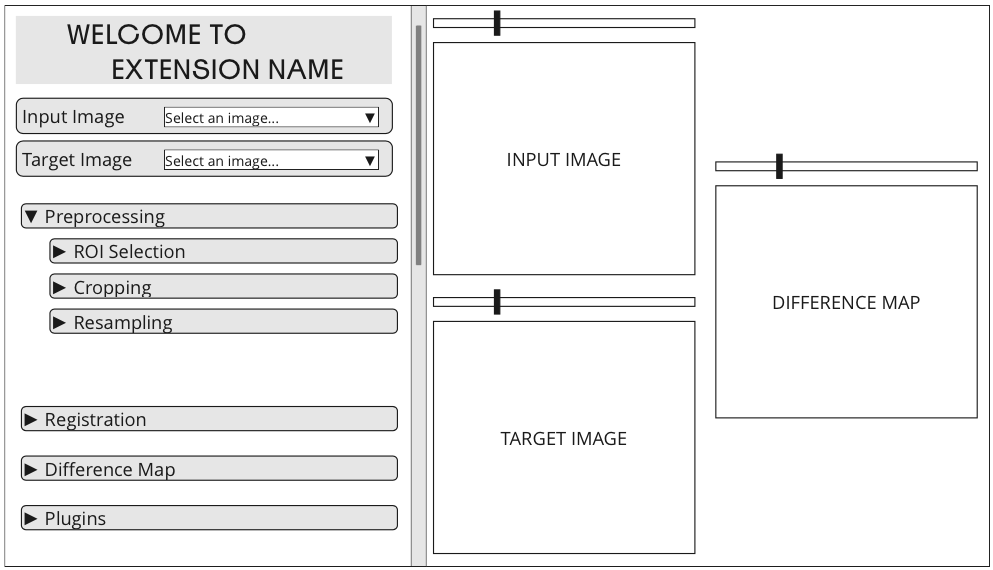
\includegraphics[width=\textwidth]{images/ui-mock-up.png}
            \caption{Maquette de 3D~Slicer ouvert sur notre module d'extension.}
            \label{fig:ui-mock-up}
        \end{figure}

        \bigskip

        Pour la \hyperref[us:preprocessing]{US I}, l'interface de prétraitements doit permettre de sélectionner l'image d'entrée, et celle de référence lorsque c'est nécessaire (blocs de sélection \textit{Input Image} et \textit{Target Image}, Figure~\ref{fig:ui-mock-up}) et de les afficher, tout comme l'image résultante (blocs d'affichage \textit{Input Image} et \textit{Target Image}, Figure~\ref{fig:ui-mock-up}).
        Ensuite, les options de prétraitement doivent inclure la sélection de ROI par seuillage, le rognage manuel et automatique, ainsi que le rééchantillonnage automatique (bouton dépliant \textit{Preprocessing}, Figure~\ref{fig:ui-mock-up}).
        Elles doivent également être paramétrables via l'interface dédiée (Figures~\ref{fig:roi-ui-mock-up},~\ref{fig:cropping-ui-mock-up} et~\ref{fig:resampling-ui-mock-up}).
        Enfin, l'interface doit afficher une prévisualisation du traitement souhaité, en temps réel.

        \begin{figure}[!ht]
            \centering
            \begin{minipage}[t]{0.3\textwidth}
                \centering
                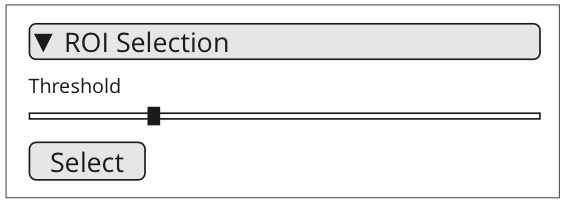
\includegraphics[width=\textwidth]{images/roi-ui-mock-up.png}
                \caption{Maquette de l'UI de sélection de ROI.}
                \label{fig:roi-ui-mock-up}
            \end{minipage}
            \hfill
            \begin{minipage}[t]{0.3\textwidth}
                \centering
                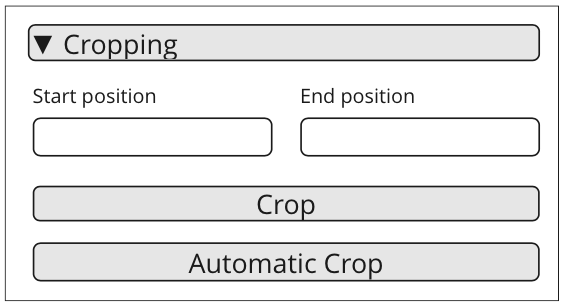
\includegraphics[width=\textwidth]{images/cropping-ui-mock-up.png}
                \caption{Maquette de l'UI de rognage.}
                \label{fig:cropping-ui-mock-up}
            \end{minipage}
            \hfill
            \begin{minipage}[t]{0.3\textwidth}
                \centering
                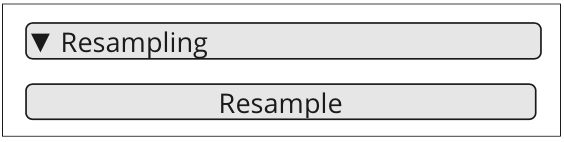
\includegraphics[width=\textwidth]{images/resampling-ui-mock-up.png}
                \caption{Maquette de l'UI de rééchantillonnage.}
                \label{fig:resampling-ui-mock-up}
            \end{minipage}
        \end{figure}

        \bigskip

        En ce qui concerne la \hyperref[us:registration]{US II}, l'interface de recalage doit non seulement permettre de sélectionner l'image à recaler et celle de référence (blocs de sélection \textit{Input Image} et \textit{Target Image}, Figure~\ref{fig:ui-mock-up}), mais elle doit aussi les afficher tout comme l'image recalée générée (blocs d'affichage \textit{Input Image}, \textit{Target Image} et \textit{Difference Map}, Figure~\ref{fig:ui-mock-up}).
        Quant aux options de recalage, elles doivent inclure des algorithmes rigides et non rigides paramétrables manuellement ou à l'aide de presets (Figure~\ref{fig:registration-ui-mock-up}).

        \begin{figure}[!ht]
            \centering
            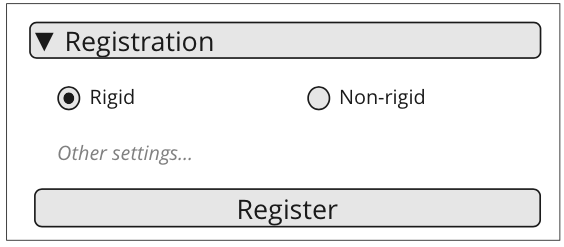
\includegraphics[width=0.4\textwidth]{images/registration-ui-mock-up.png}
            \caption{Maquette de l'UI de recalage.}
            \label{fig:registration-ui-mock-up}
        \end{figure}

        \newpage

        Quant à la \hyperref[us:diff-map]{US III}, l'interface de calcul de la carte de différence doit permettre de sélectionner les images à comparer (blocs de sélection \textit{Input Image} et \textit{Target Image}, Figure~\ref{fig:ui-mock-up}) mais aussi d'afficher la carte calculée dans la vue (bloc d'affichage \textit{Difference Map}, Figure~\ref{fig:ui-mock-up}).
        En outre, les options de calcul de la carte de différence doivent inclure la possibilité de calculer la différence voxel-à-voxel ou par gradients, et de spécifier l'utilisation de patchs (Figure~\ref{fig:diff-map-ui-mock-up}).

        \begin{figure}[!ht]
            \centering
            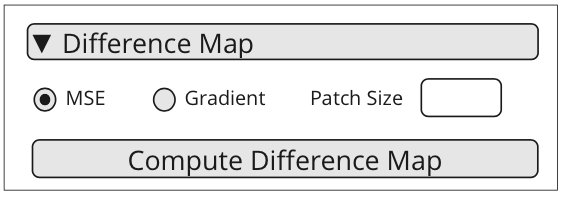
\includegraphics[width=0.4\textwidth]{images/diff-map-ui-mock-up.png}
            \caption{Maquette de l'UI de génération de carte de différence.}
            \label{fig:diff-map-ui-mock-up}
        \end{figure}

        \bigskip

        Pour finir, pour la \hyperref[us:plugins]{US IV}, l'interface de développement doit permettre l'importation d'une interface XML et d'un script Python pour une utilisation en tant que plugin.

        Ensuite, ces plugins doivent être intégrables dans le logiciel principal et accessibles via une interface dédiée (Figure~\ref{fig:plugins-ui-mock-up}).
        Enfin, les plugins doivent être compatibles avec les autres fonctionnalités du logiciel, en s'intégrant au sein de l'architecture de l'extension.

        \begin{figure}[!ht]
            \centering
            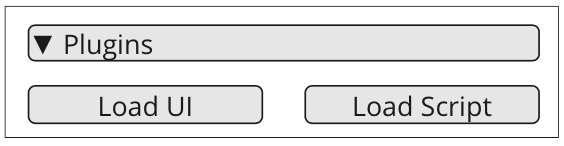
\includegraphics[width=0.4\textwidth]{images/plugins-ui-mock-up.png}
            \caption{Maquette de l'UI d'intégration de plugins.}
            \label{fig:plugins-ui-mock-up}
        \end{figure}

        \bigskip

        Pour une vision plus globale et concise des US et de leurs critères d'acceptabilité, voir le tableau récapitulatif (Section~\ref{sec:annexes}, Figure~\ref{fig:us-recap}).
    }

    \newpage
}

% Tests
{
    \section{Tests}
    \label{sec:testing}

    Durant le processus de développement du projet, les tests ont été la base de l'implémentation de chacune des User~Stories. Deux types de tests sont à mettre en évidence dans ce projet.

    % Monkey Testing
    {
        \bigskip
        \subsection{Monkey Testing}
        \label{subsec:monkey-testing}

        Le premier type de tests à prendre en compte concerne la robustesse de l'interface graphique (UI). L'idée ici est d'être certain que son utilisation permet de réaliser les appels aux algorithmes souhaités, avec les paramètres adéquats, tout en assurant le bon fonctionnement du logiciel et de l'extension. On souhaite donc vérifier qu'aucun bug n'apparaît lors de la manipulation de l'UI.

        \bigskip

        Pour ce faire, chaque tâche dédiée à l'UI a été testée avec la méthode du Monkey Testing. En d'autres termes, chaque élément de l'UI est utilisé dans différentes conditions d'utilisation, allant de réalistes à aberrantes pour couvrir tous les cas possibles, en cherchant la présence de bugs. Chacun des bugs mis en évidences grâce à cette méthode ont été traités de manière à assurer une utilisation stable en toutes conditions.
    }

    % Unit Testing
    {
        \bigskip
        \subsection{Unit Testing}
        \label{subsec:unit-testing}

        La seconde gamme de tests à considérer s'applique aux appels d'algorithmes, écrits manuellement ou via les différentes bibliothèques utilisées dans le projet (\textit{SimpleITK} et \textit{Elastix}), avec les différents paramètres prévus. Ces fonctionnalités sont testées à l'aide de tests unitaires précisés par la suite.

        \bigskip

        Pour mettre en place ces tests, nous tirons avantage de la classe \texttt{ScriptedLoadableModuleTest} dont 3D~Slicer dispose comme présenté en Section~\ref{subsubsec:extension-module}. En surchargeant la méthode \texttt{runTest}, nous pouvons configurer les appels aux méthodes individuelles qui testent chaque fonctionnalité lorsqu'on clique sur le bouton \textit{Reload \& Test}.

        En outre, pour faciliter l'utilisation de cette classe de test, nous avons implémenté les méthodes utilitaires \texttt{resourcePath} et \texttt{assertVolumeEqual}. Elles permettent respectivement de récupérer le chemin absolu jusqu'à un fichier donné, et de vérifier que deux \textit{VTK Volume} sont égaux.

        % Prétraitements
        {
            \subsubsection{Prétraitements}
            \label{subsubsec:preprocessing-unit-testing}

            % Sélection de ROI
            {
                \subsubsubsection{Sélection de ROI}
                \label{subsubsubsec:roi-selection-unit-testing}

                \method{test\_roi\_selection}
                \label{method:test_roi_selection}

                Dans le cadre du test unitaire de la sélection de ROI, deux méthodes sont utilisées à la suite dans la classe \texttt{Widget}, \texttt{create\_mask} et \texttt{select\_roi}. Elles sont toutes les deux appeler dans ces tests, le résultat final étant testé en le comparant au résultat attendu généré préalablement.

                \bigskip

                Tout d'abord, une image 3D a été générée via \textit{SimpleITK} et \textit{NumPy}. Cette image correspond à une sphère dont les voxels intérieurs valent 2, sur un fond dont les voxels valent 0. Elle est aléatoirement bruité avec des valeurs de 1 afin de rendre le seuillage moins évident (Figure~\ref{fig:test-roi-selection-volume}).  Une version non bruitée est également générée avec des valeurs de 1 à l'intérieur de la sphère. Cette version correspond à la ROI de la sphère uniquement (Figure~\ref{fig:test-roi-selection-roi}).

                Ainsi, en faisant une sélection de ROI par seuillage avec une valeur de seuillage de 2, on devrait sélectionner uniquement la sphère (Figure~\ref{fig:test-roi-selection-preview-2}), et non le fond ni le bruit (Figure~\ref{fig:test-roi-selection-preview-1}).

                \begin{figure}[!p]
                    \centering

                    \begin{minipage}[t]{0.45\textwidth}
                        \centering
                        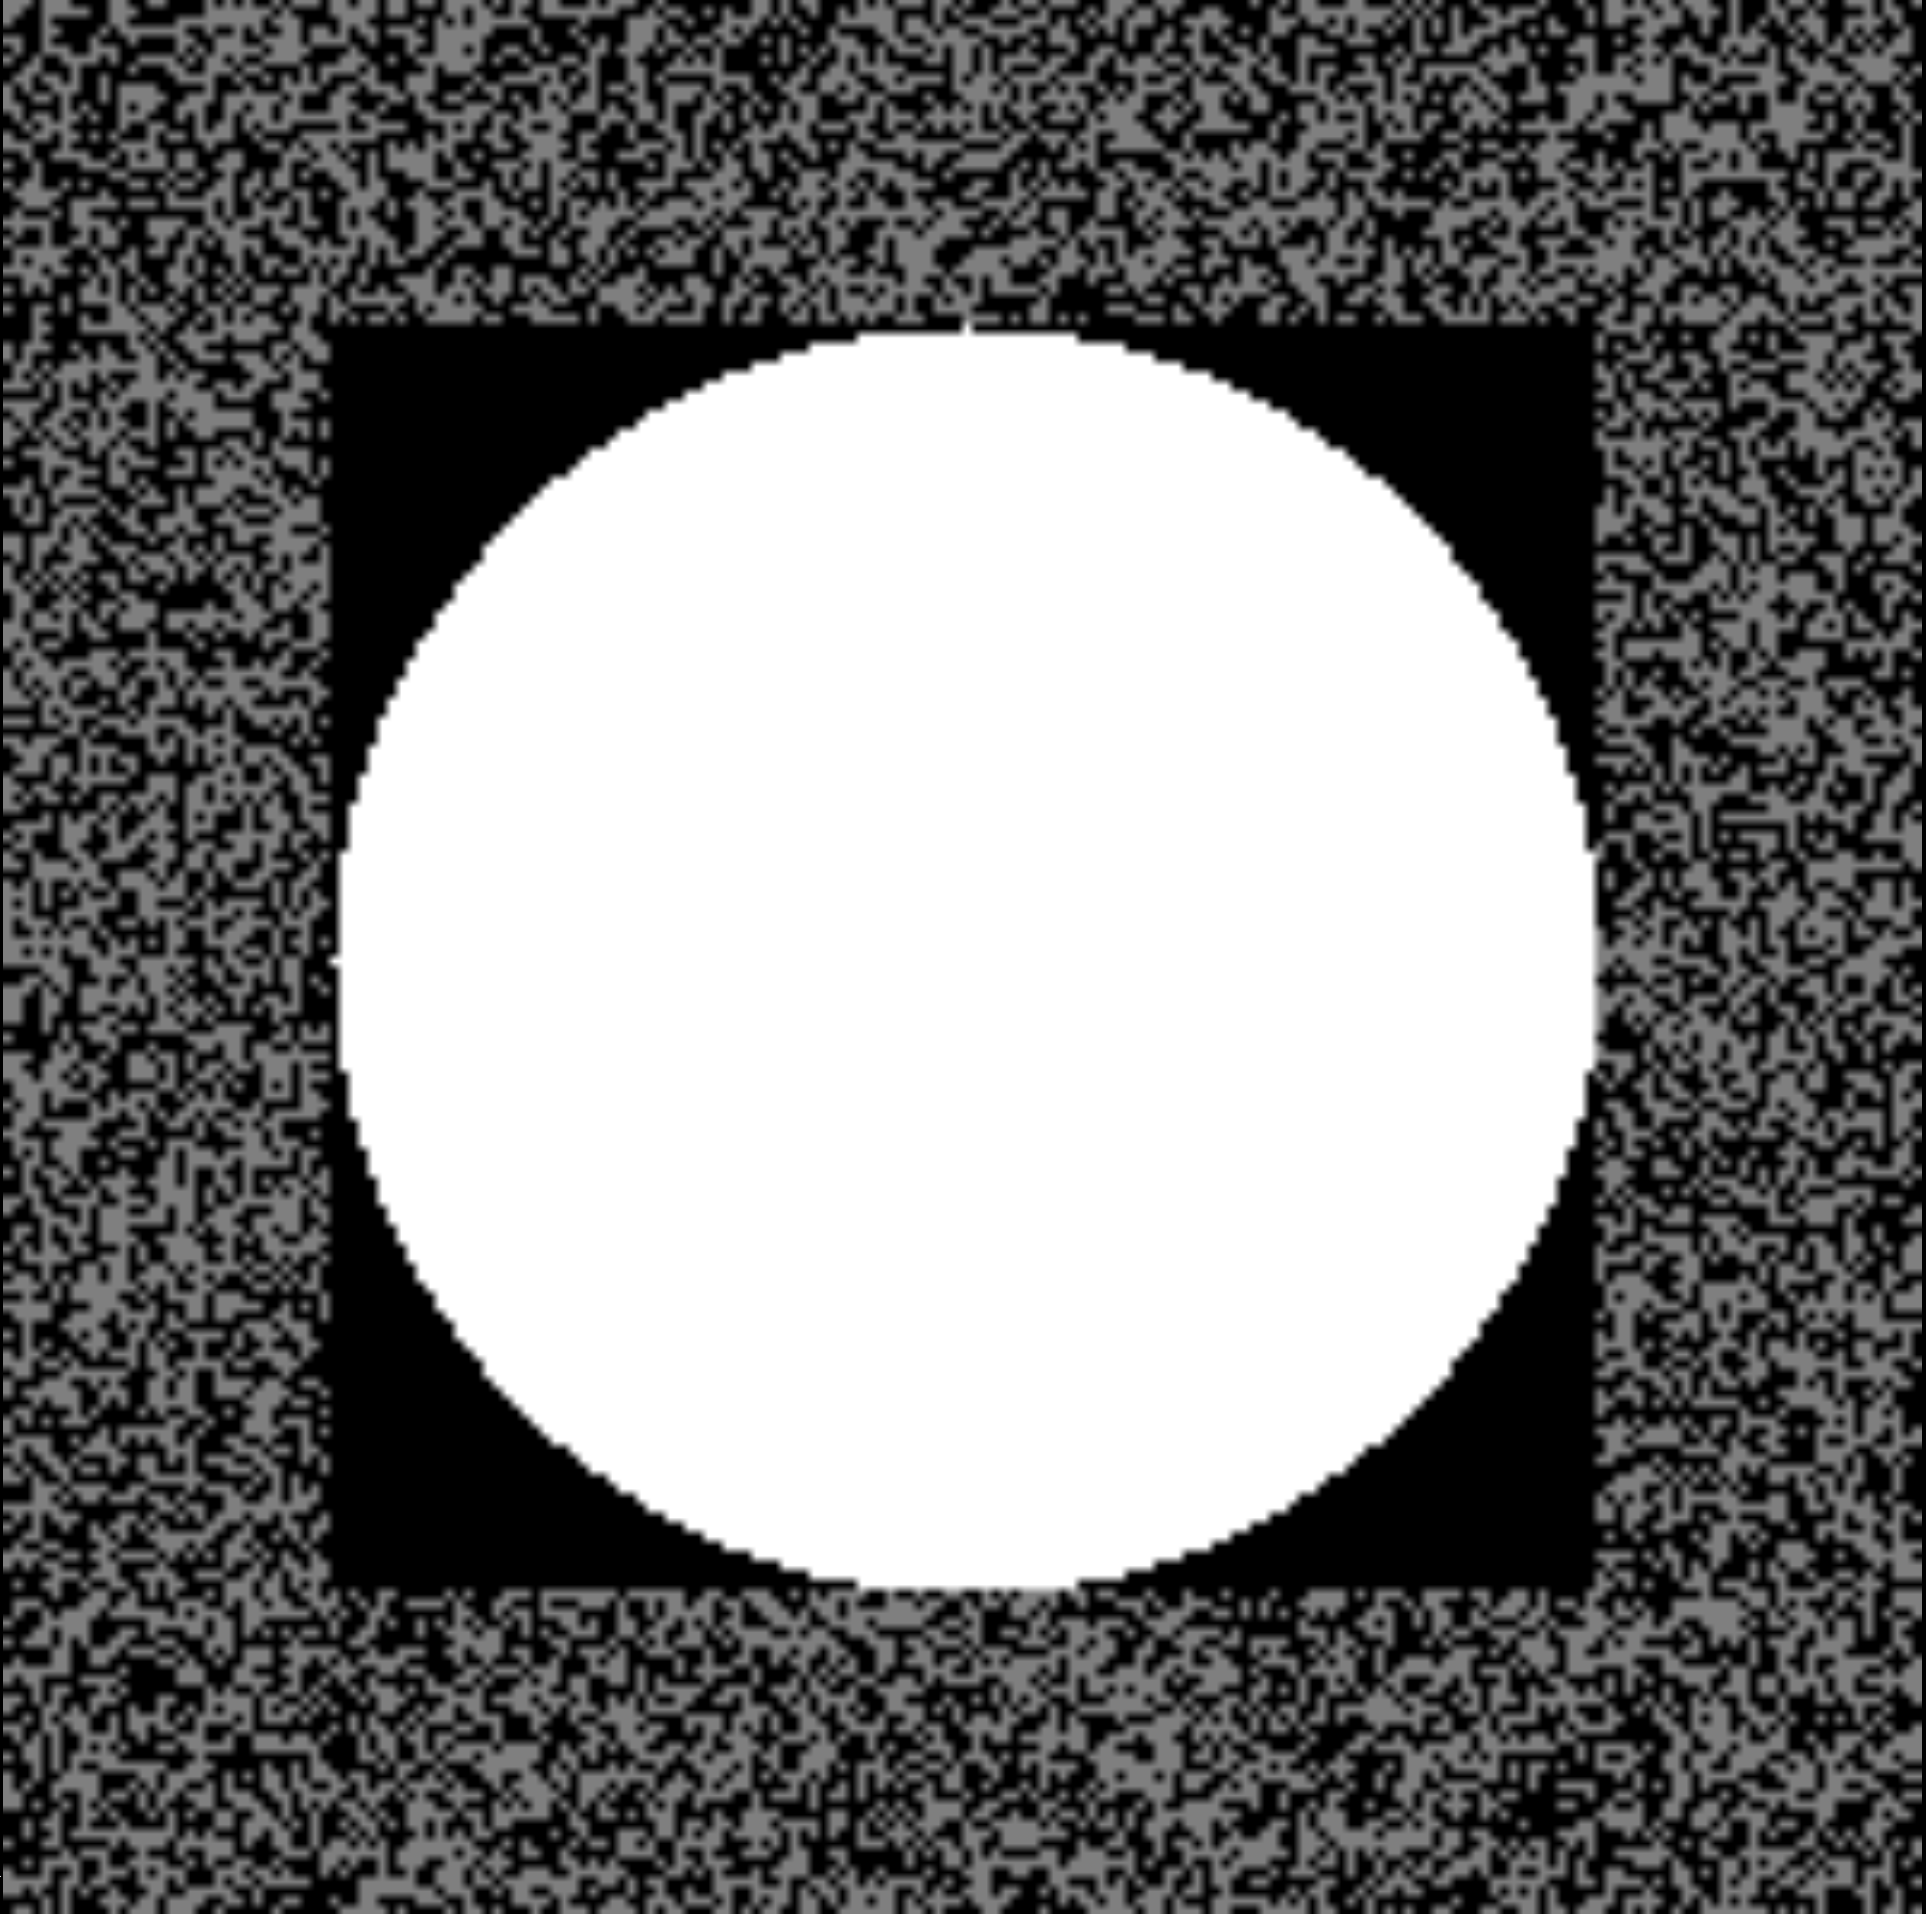
\includegraphics[width=\textwidth]{images/test-roi-selection-volume.png}
                        \caption{Image générée de l'image bruitée de la sphère (image d'entrée).}
                        \label{fig:test-roi-selection-volume}
                    \end{minipage}
                    \hfill
                    \begin{minipage}[t]{0.45\textwidth}
                        \centering
                        
\includegraphics[width=\textwidth]{images/test-roi-selection-roi.png}
                        \caption{Image générée de la ROI de la sphère, attendue après le calcul.}
                        \label{fig:test-roi-selection-roi}
                    \end{minipage}

                    \bigskip\bigskip\bigskip

                    \begin{minipage}[t]{0.45\textwidth}
                        \centering
                        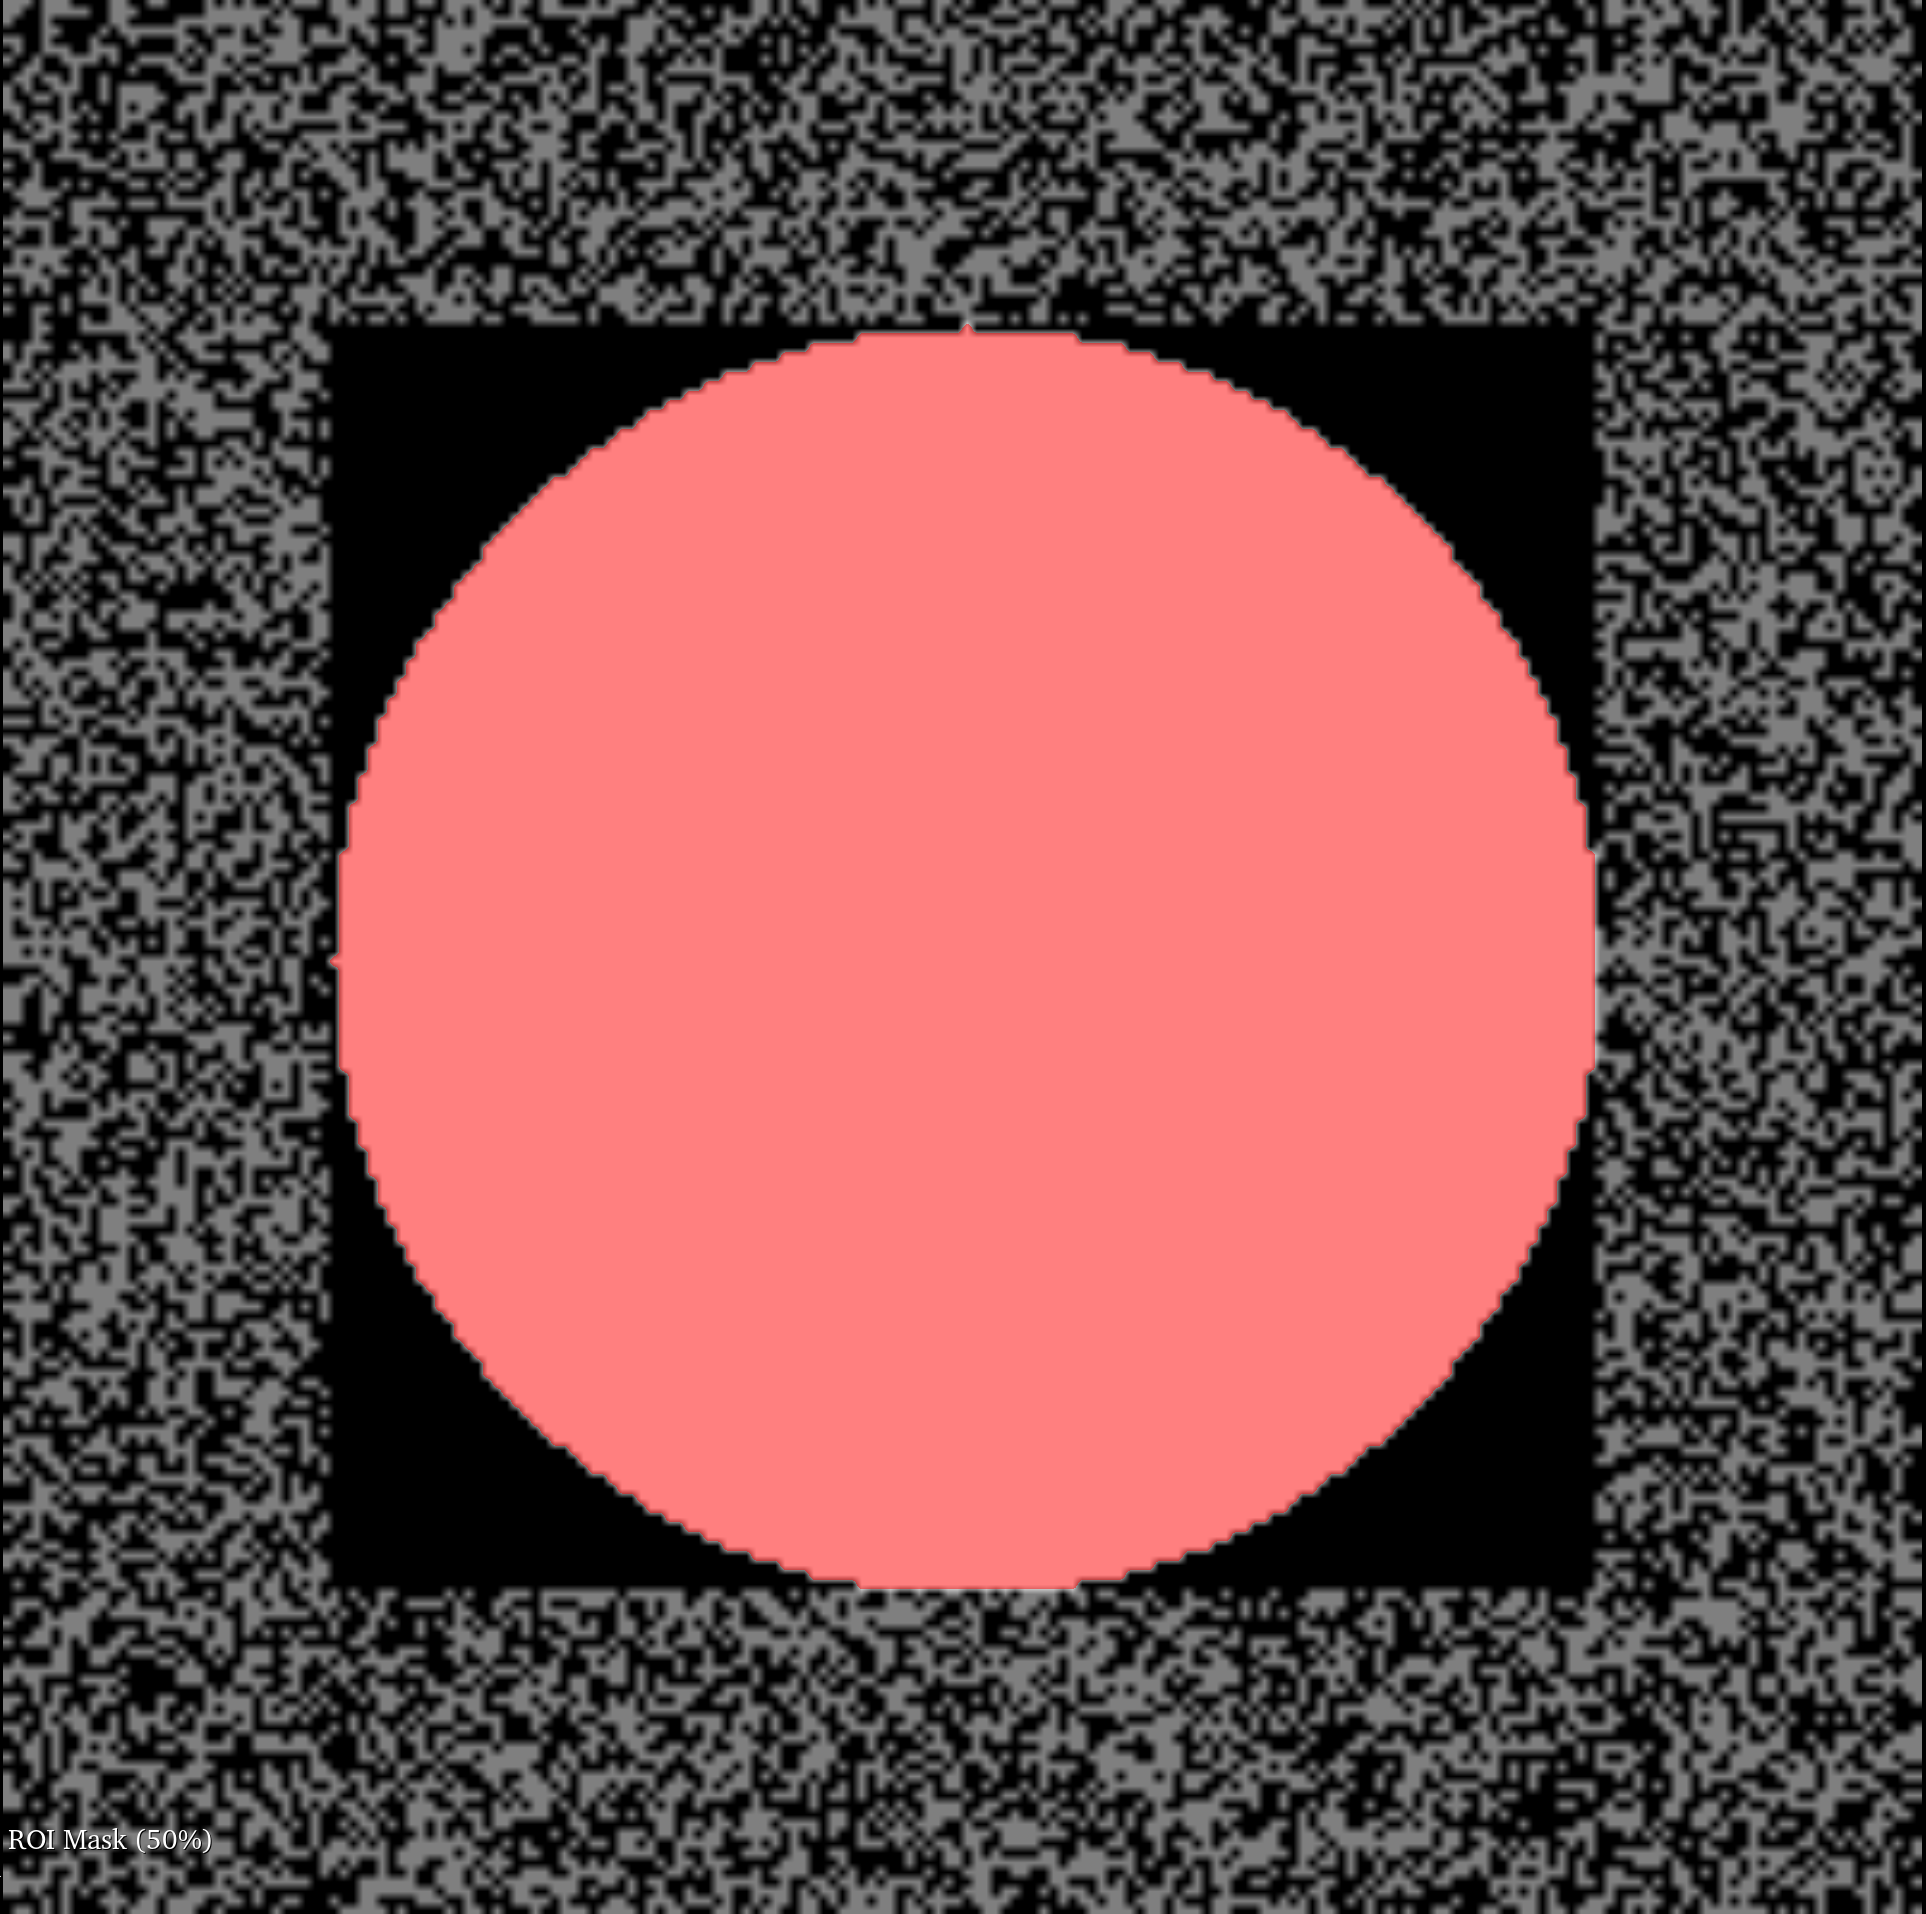
\includegraphics[width=\textwidth]{images/test-roi-selection-preview-2.png}
                        \caption{prévisualisation de la ROI calculée avec un seuillage à 2.}
                        \label{fig:test-roi-selection-preview-2}
                    \end{minipage}
                    \hfill
                    \begin{minipage}[t]{0.45\textwidth}
                        \centering
                        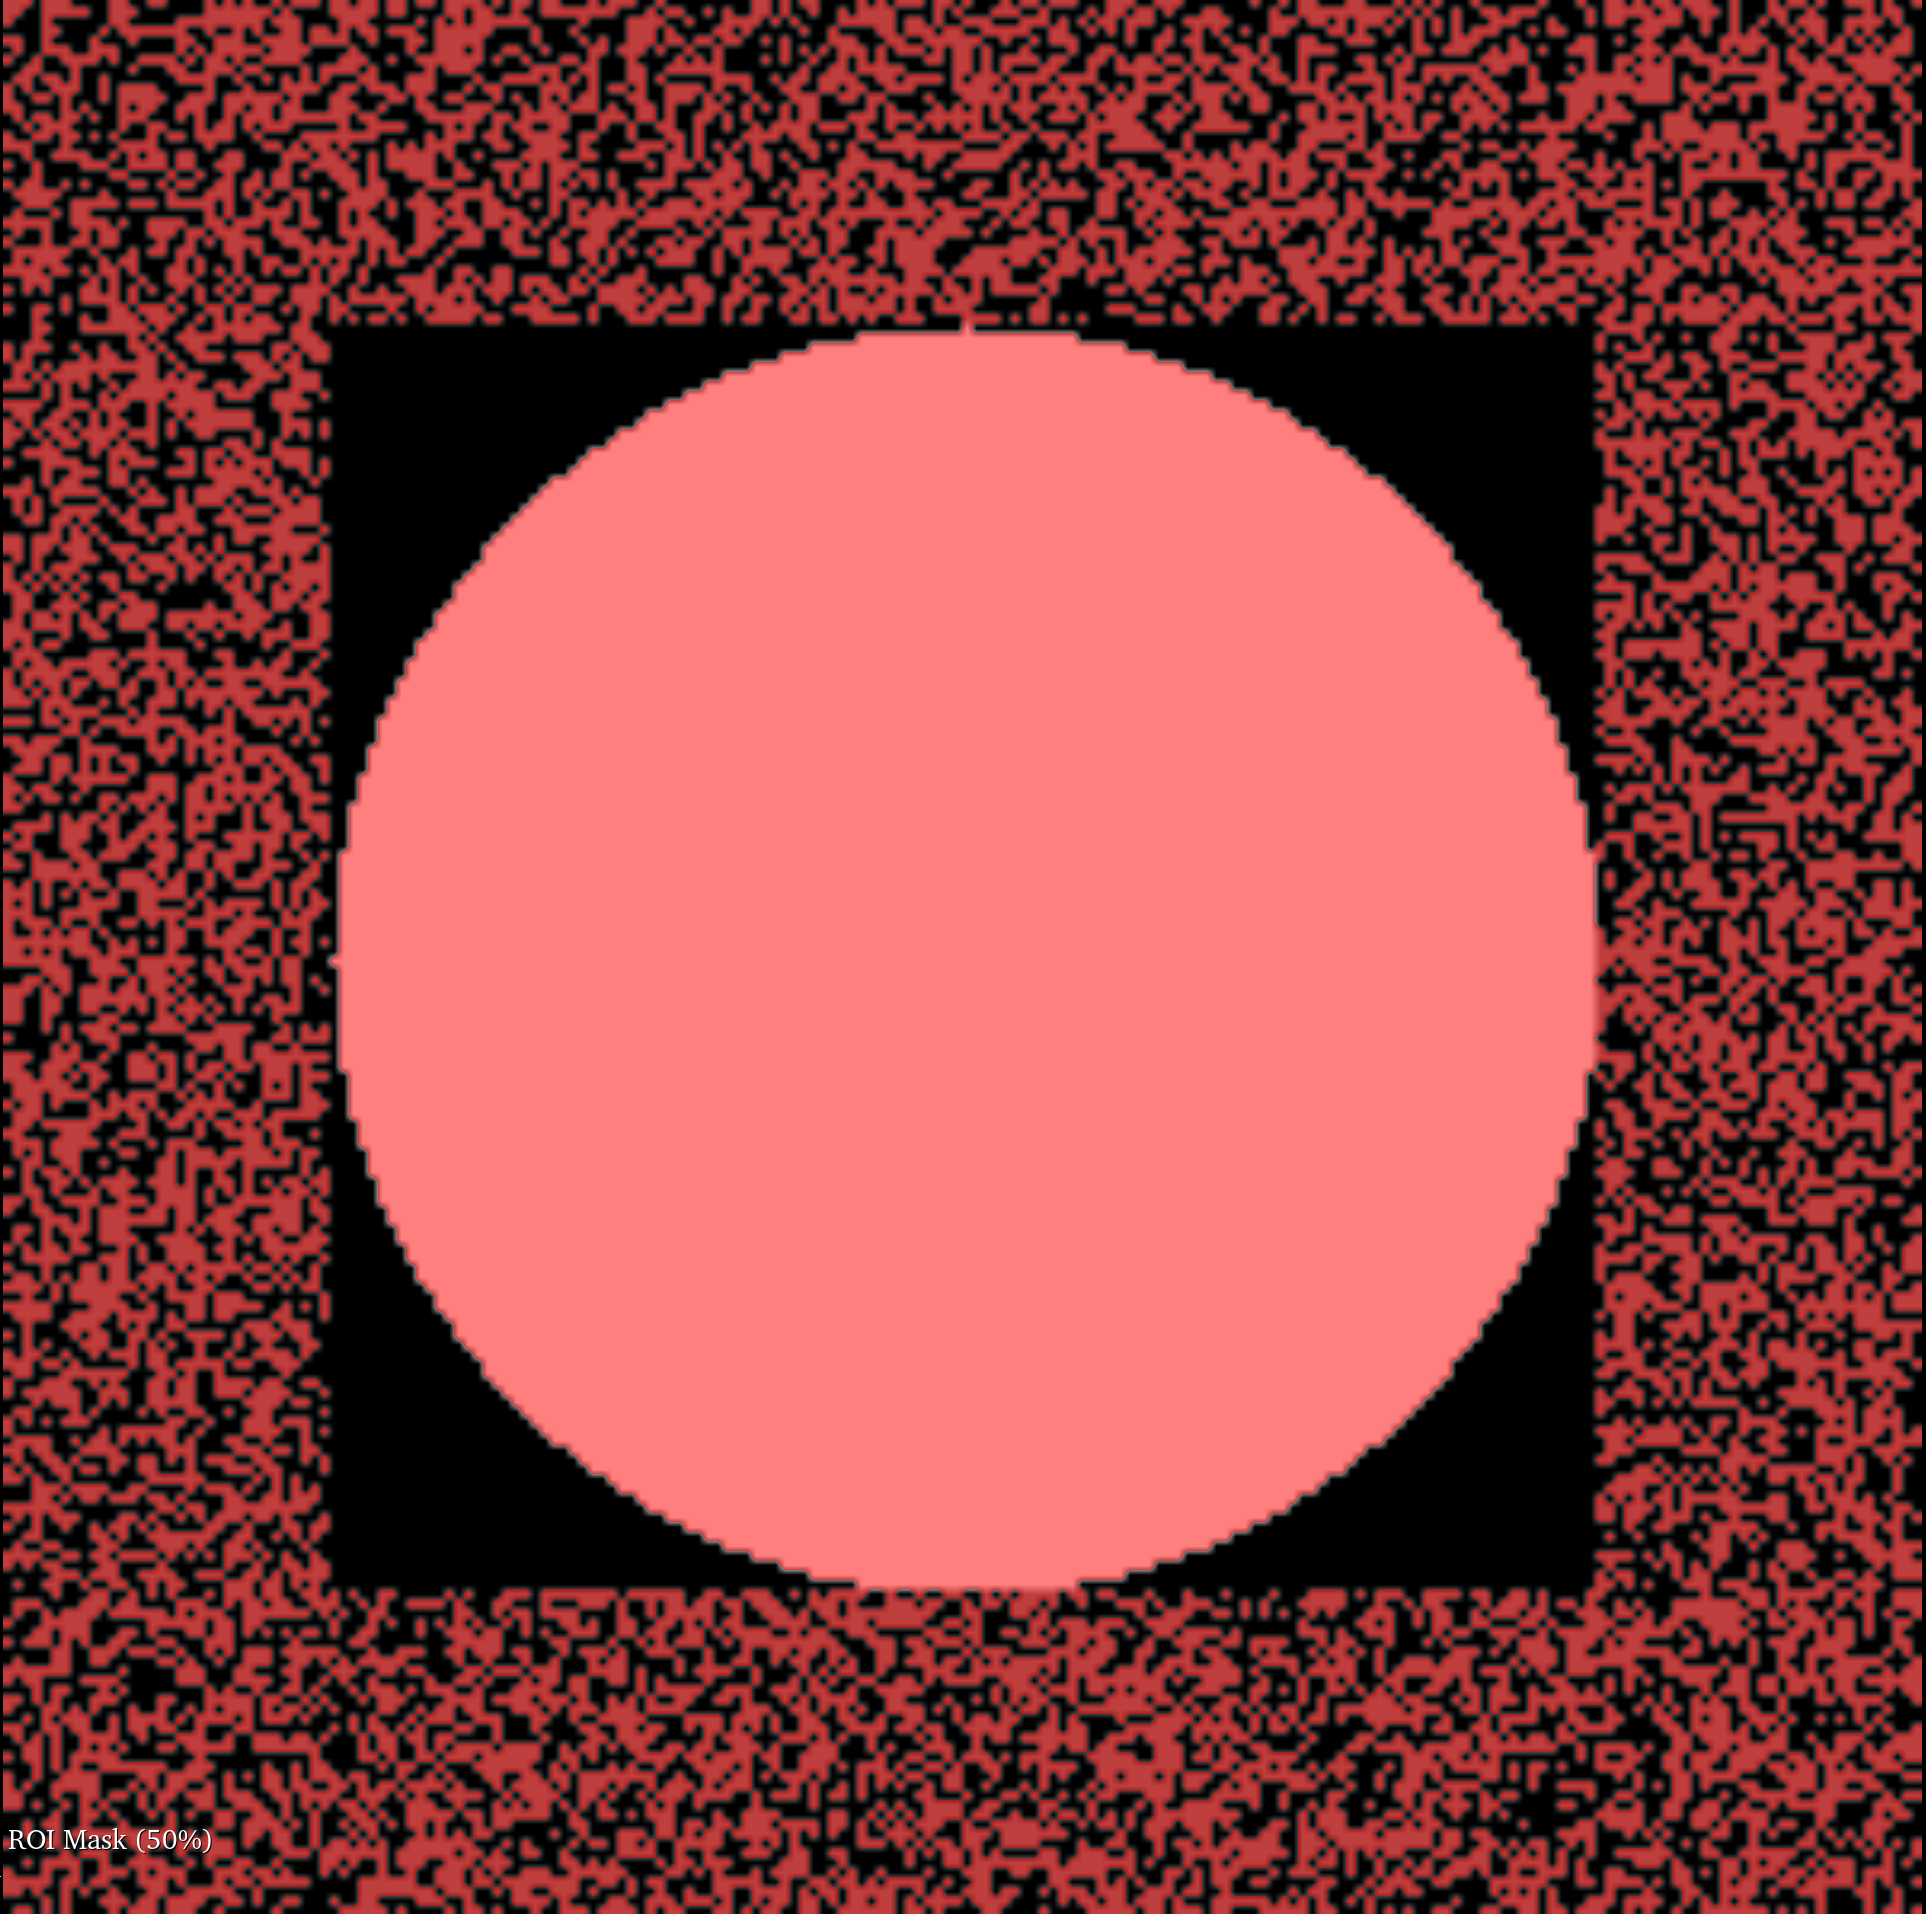
\includegraphics[width=\textwidth]{images/test-roi-selection-preview-1.png}
                        \caption{prévisualisation de la ROI calculée avec un seuillage à 1.}
                        \label{fig:test-roi-selection-preview-1}
                    \end{minipage}
                \end{figure}
            }

            % Rognage
            {
                \bigskip
                \subsubsubsection{Rognage}
                \label{subsubsubsec:cropping-unit-testing}

                \method{test\_manual\_cropping}
                \label{method:test_manual_cropping}

                Pour le test unitaire du rognage manuel qui teste la méthode \texttt{crop}, la première étape consiste à créer et stocker une image \textit{VTK Volume} avec 3D~Slicer. Cette image qui constituera l'image attendue, à partir d'une boîte englobante valide définie arbitrairement.

                Puis dans la méthode, on commence par vérifier que des paramètres invalides résultent en une erreur en ajoutant ou soustrayant une grande à valeur à la boîte englobante définie au préalable.

                Finalement, on crée une image à partir des paramètres valides et on s'assure qu'elle est identique à l'image attendue.

                \bigskip
                \method{test\_automatic\_cropping}
                \label{method:test_automatic_cropping}

                Le test unitaire pour le rognage automatique est très similaire à celui du rognage manuel. Il est construit de la même manière à la seule différence qu'il est également nécessaire de créer un \textit{VTK Volume} représentant la ROI, et qu'il est question de tester les marges au lieu d'une boîte englobante.

                Par ailleurs l'image de la ROI est créée à partir de notre extension. En effet, ce test admet que la sélection de ROI est fonctionnelle et, qu'on ne teste ici que le rognage automatique.
            }

            % rééchantillonnage
            {
                \bigskip
                \subsubsubsection{rééchantillonnage}

                \method{test\_resampling}
                \label{method:test_resampling}

                La fonctionnalité de rééchantillonnage est testée en prenant plusieurs couples d'images avec des résolutions spatiales différentes, et en vérifiant que les deux aient la même en sortie.

                \bigskip

                Dans cette optique, plusieurs couples d'images d'entrée/cible sont définis grâce aux images de test. Pour chacun de ces couples, la méthode \texttt{Logic.crop} est appelée pour rééchantillonner l'image d'entrée en fonction de l'image cible. On vérifie alors que l'image en sortie de cette méthode est bien rééchantillonnée.
            }
        }

        % Recalage
        {
            \subsubsection{Recalage}
            \label{subsubsec:registration-unit-testing}

            Les tests peuvent être exécutés indépendamment de 3D~Slicer, il suffit de lancer le script dédié \texttt{test\_registration.py} disponible dans le dossier \textit{Scripts/Registration}. Les tests s'effectuent sur un jeu de données disponibles dans le dossier \textit{TestData} déjà utilisé pour les tests précédents. Il contient entre autre une image cible (référence fixe) \textit{RegLib\_C01\_MRMeningioma\_1}, une image à recaler \textit{RegLib\_C01\_MRMeningioma\_2}, une image rééchantillonnée, une image résultat d'un recalage affine, et des fichier .tfm symbolisant les résultats des transformations attendues, ce sont sur ces transformations que se font la plupart des tests.

            Avant de pouvoir s'attaquer aux tests de chaque scripts. Il est nécessaire de tester les méthodes auxiliaires du fichier \textit{Utilities.py} incessamment employés dans le code des méthodes de recalage.

            \bigskip
            \method{test\_select\_metrics\_1}

            La première méthode testée, intitulée \textit{select\_metrics}, attache une métrique à l'objet \textit{ImageRegistrationMethod}. Un recalage basique avec les méthodes de la bibliothèque SimpleITk résulte en un objet transform, directement comparé à un autre objet transform obtenue de manière similaire, mais la métrique n'a pas été sélectionné avec la fonction testée. Les transforms sont comparées à l'aide de leur coefficients. La métrique sélectionnée ici se nomme \textit{Mattes Mutual Information}

            \bigskip
            \method{test\_select\_metrics\_2}

            Ce test reprend les grandes lignes du test ci-dessus, la seule différence se situe dans la métrique testée, ici \textit{Mean Squares}. Les objets transforms sont comparés de la même manière.

            \bigskip
            \method{test\_select\_metrics\_3}

            Même chose qu'au dessus, mais cette fois nous testons la métrique \textit{Joint Histogram Mutual Information}.

            \bigskip
            \method{test\_select\_metrics\_4}

            Même chose qu'au dessus, mais cette fois nous testons la métrique \textit{Correlation}.

            \bigskip
            \method{test\_select\_metrics\_5}

            Ce test unitaire contient un ensemble de tests négatifs sur la méthode \textit{select\_metrics}. Elle affirme aussi que différentes métriques ne donnent pas les mêmes résultats pour un jeu de paramètres équivalent. Pour cela on compare les transforms résultants des recalages.

            \bigskip
            \method{test\_select\_interpolator}

            Ce test unitaire affirme la robustesse de la méthode \textit{select\_interpolator}. Pour cela, la méthode testée fixe un interpolateur sur un objet \textit{ImageRegistrationMethod}, puis on récupère l'interpolateur avec la méthode de la bibliothèque \textit{GetInterpolator}, et il y a une simple assertion entre l'interpolateur sélectionné et l'interpolateur récupéré. Tous les interpolateurs disponibles dans l'extension sont testés de cette manière.

            \bigskip
            \method{test\_select\_optimizer\_1}

            Approche analogue à plus haut, la méthode \textit{select\_interpolator} met au point l'interpolateur passé en paramètre à un objet de type \textit{ImageRegistrationMethod}, les méthodes de la bibliothèque SITK prennent le relais pour élaborer un objet de type transform, un autre objet \textit{ImageRegistrationMethod} est créé, cette fois sans utiliser la méthode testée, et s'exécute pour créer un objet transform, que l'on va comparer avec celui précédemment calculé. Cette méthode teste l'optimiseur \textit{Gradient Descent}

            \bigskip
            \method{test\_select\_optimizer\_2}

            La même méthode de test unitaire du dessus est reprise, cette fois ci, l'optimiseur \textit{Exhaustive} est mis à l'épreuve. Nous comparons les coefficients des deux objets \textit{transforms} calculés, avec un delta de 0.01.

            \bigskip
            \method{test\_select\_optimizer\_3}

            \textit{LBFGSB} mis au banc d'essais sur ce test unitaire. Nous comparons les coefficients des deux objets \textit{transforms} calculés, avec un delta de 0.0001.

            \bigskip
            \method{test\_select\_optimizer\_4}

            Ici, des tests négatifs sont effectués avec les valeurs utilisateurs insensées. ce genre de valeurs ne peuvent arriver puisque l'UI prévient ce genre de comportement.

            \bigskip
            \method{test\_rigid\_registration\_1}

            Ce premier test exécute la méthode \textit{rigid\_registration} du fichier \textit{Rigid.py}, récupère la transformation obtenue et compare la transformation attendue du fichier \textit{expected\_transform\_1.tfm}. Ce sont les coefficients de la transformations qui sont comparés. Chaque tests rigides utilisent différents optimiseurs et différents paramètres pour prouver la robustesse du code.

            \bigskip
            \method{test\_rigid\_registration\_2}

            Ce test réalise la même chose, mais avec l'optimiseur exhaustif, et le fichier \textit{expected\_transform\_2.tfm}. A noter que pour le recalage rigide, la reproductibilité des résultats est possible, mais lors du passage au non rigide, il n'est pas possible d'avoir exactement les mêmes résultats. De ce fait nous ne comparerons plus les coefficients.

            \bigskip
            \method{test\_rigid\_registration\_3}

            Comme pour le premier et deuxième test, nous vérifions que la transformation résultante n'est pas vide. Cette fois-ci l'optimiseur LBFGSB est utilisé, et nous comparons au fichier contenant le résultat attendu \textit{expected\_transform\_3.tfm}.

            \bigskip
            \method{test\_non\_rigid\_registration\_1}

            Les tests de recalage non rigide s'exécutent avec la méthode \textit{non\_rigid\_registration} disponible dans le fichier \textit{NonRigid.py}. Ce premier test utilise la méthode B-Spline avec l'optimiseur LBFGSB. La comparaison de \textit{expected\_transform\_4.tfm} avec les coefficients rassure sur le fait que la méthode fonctionne, même si les résultats ne sont pas tout à fait les mêmes à cause de la particularité du non rigide à déformer.

            \bigskip
            \method{test\_non\_rigid\_registration\_2}

            La descente de gradient et le recalage non rigide n'assurent pas une reproductibilité, malgré tout, il y a comparaison du nombre de coefficients. On s'assure aussi que la transformation n'est pas vide.

            \bigskip
            \method{test\_non\_rigid\_registration\_3}

            Ce test vérifie que l'utilisation d'un vecteur \textit{Scale Factor} avec l'optimiseur LBFGSB lève bien une exception. Il n'y a pas plus de tests négatifs sur ces méthodes puisque les \textit{observers} attachés à l'UI préviennent les entrées utilisateurs incohérentes.

            \bigskip
            \method{test\_demons\_registration\_1}

            C'est un simple test unitaire qui vérifie l'exécution de la méthode \textit{non\_rigid\_registration} avec le filtre général Demons. Comme attendu, puisque les images n'ont pas été rééchantillonnées, l'objet transform est vide.

            \bigskip
            \method{test\_demons\_registration\_2}

            Le test unitaire 2 exécute la même méthode que le test précédent. L'exactitude de la méthode est testée via l'exécution dans le test d'une méthode Demons depuis la bibliothèque avec les mêmes paramètres. Les coefficients sont comparés avec un delta de 0.01, puisque la reproductibilité n'est pas assurée.

            \bigskip
            \method{test\_demons\_registration\_3}

            Ce test unitaire sélectionne Diffeomorphic Demons, et comme prévu donne un résultat vide même avec une image rééchantillonnée, en effet ce filtre a besoin d'un recalage affine avant d'être utilisée, comme les autres filtres Demons. La méthode compare les coefficients avec la méthode de la bibliothèque directement, avec un delta de 1 pour les coefficients non fixes, et un delta de 0.1 pour les coefficients fixes.

            \bigskip
            \method{test\_demons\_registration\_4}

            Ce test est similaire au test précédent, seul le filtre Demons est altéré, c'est avec le filtre Fast Symmetric Forces Demons que la méthode de recalage s'exécute. Comme auparavant, l'objet \textit{transform} est comparé à un autre objet \textit{transform} directement obtenue depuis la bibliothèque, cette fois avec un delta de 0.01 pour tous les coefficients.

            \bigskip
            \method{test\_demons\_registration\_5}

            Ce dernier test sur la partie Demons reprend la même structure que son test antécédent. Cette fois Symmetric Forces Demons est testé, les coefficients sont comparés avec un delta de 0.01 chacun.
        }

        % Carte de différence
        {
            \subsubsection{Carte de différence}
            \label{subsubsec:difference-map-unit-testing}

            \method{test\_difference\_map}

            Le test se décompose en trois parties, une pour la différence de valeur absolue, une pour la différence de gradient, et enfin une dernière pour le noyau de convolution. Pour tester les fonctions de la carte de différence, nous avons créé deux images de référence de type \textbf{vtkMRMLScalarVolumeNode} à partir de tableau numpy de taille [3x3x3] appelé \textit{imageData1} et \textit{imageData1}, ces deux tableaux sont remplis de 0. Il suffit d'appeler la méthode \textit{difference\_map}, et comparer l'image de sortie et l'image attendu.

            \subsubsubsection{Différence de la valeur absolue}

            Pour la différence de la valeur absolue, pour un voxel donné, sur les deux images d'entrées, comparer la valeur attendu. Dans notre cas nous avons juste mis sur \textit{imageData1} un voxel à 0 et \textit{imageData2} un voxel à 1. La valeur attendus de celui-ci est 1 car la valeur absolue de $|0 - 1|$ est 1.

            \subsubsubsection{Différence du gradient}

            Pour ce test, nous avons juste précalculé la valeur attendu du tableau grâce à la méthode de NumPy \texttt{np.gradient}. Ça nous permet aussi de savoir si la fonction arrive bien à passer de \textbf{vtkMRMLScalarVolumeNode} à \texttt{np.array} et inversement.

            \subsubsubsection{Noyau de convolution}

            Enfin, pour tester le noyau de convolution sur le voxel donné [1,1,1], nous avons crée une différence de 0.5, qui se traduit en une différence de 1 après normalisation. Le résultat attendu est le voxel [1,1,1] toujours sur une valeur de 1. Et ses voxels voisins (car noyau de 3) la moyenne des voxels contenu dans le noyau.
        }
    }

    \newpage
}

% Implémentation
{
    \section{Implémentation}
    \label{sec:implementation}

    % Architecture générale
    {
        \bigskip
        \subsection{Implémentation globale}
        \label{subsec:global-implementation}

        % Module d'extension
        {
            \subsubsection{Module d'extension}
            \label{subsubsec:extension-module}

            3D~Slicer dispose d'un outil permettant de générer un modèle d'extension vide depuis son interface même. Une extension peut être composée d'un ou plusieurs modules. Un module est une composante de l'extension qui sera affichée dans 3D~Slicer indépendamment des autres --- attention à ne pas confondre un module d'extension de 3D~Slicer et un module Python qui correspond plus simplement à un script Python que l'on peut importer.

            Dans notre cas, nous devons n'utiliser qu'un seul module d'extension afin de regrouper toutes les fonctionnalités au sein d'une interface minimale. Un seul script Python sera alors nécessaire pour intégrer à notre extension le module.

            \bigskip

            Le module d'extension est composé de quatre classes qui héritent chacune d'une classe mère appropriée provenant de 3D~Slicer. En effet, \texttt{ScriptedLoadableModule} est le module Python de 3D~Slicer contenant les quatre classes à implémenter via des classes filles. Dans notre cas, le module est nommé \textit{Custom~Registration}. Les quatre classes du module d'extension défini par le script \texttt{CustomRegistration.py} seront alors les suivantes.

            \bigskip
            \method{CustomRegistration(ScriptedLoadableModule)}

            Classe principale définissant le module d'extension par un titre, des catégories, des dépendances potentielles, des collaborateurs, un texte d'aide informatif, un texte de reconnaissances et remerciements, et d'autres propriétés optionnelles. Son but est d'intégrer le module d'extension dans le logiciel et de le rendre exploitable en liant les trois autre classes à 3D~Slicer.

            \bigskip
            \method{CustomRegistrationLogic(ScriptedLoadableModuleLogic)}

            Classe abrégée \texttt{Logic} par la suite, dédiée aux algorithmes et calculs, ne manipulant pas l'UI ni la scène de 3D~Slicer. Les méthodes sont faites pour être appelées par la classe suivante.

            \bigskip
            \method{CustomRegistrationWidget(ScriptedLoadableModuleWidget)}

            Classe abrégée \texttt{Widget} par la suite, dédiée au lien entre l'UI et les algorithmes implémentés. Elle manipule la scène de 3D~Slicer, interagit avec l'UI du panneau de traitements et exploite les algorithmes définis dans la classes \texttt{Logic}.

            \bigskip
            \method{CustomRegistrationTest(ScriptedLoadableModuleTest)}

            Classe abrégée \texttt{Test} par la suite, dédiée à l'implémentation des tests unitaires du module d'extension. Elle peut être appelée directement depuis 3D~Slicer afin de lancer les tests unitaires.

            \bigskip

            \textbf{Nota Bene} L'UI du panneau de configuration, manipulée par la classe \texttt{Widget}, est simplement définie par le fichier de ressource \texttt{Panel.ui}. Depuis les maquettes esquissées lors du développement du projet (Section~\ref{subsec:acceptance-criteria}), elle a été mise en jour en fonction des nouveaux besoins à chaque étape.
        }

        % Architecture générale
        {
            \subsubsection{Architecture générale}
            \label{subsubsec:general-architecture}

            Dans 3D~Slicer, une image 3D est stockée dans un objet de type volume de la bibliothèque VTK. La scène correspond à l'environnement dans lequel les différents volumes évoluent. Autrement dit, lorsqu'un volume \texttt{volume} est créé, pour qu'il soit détecté par le logiciel, il doit être intégré à la scène via une méthode de 3D~Slicer~: \texttt{mrmlScene.AddNode(volume)}. Il en est de même pour la suppression. Supprimer les références au volume ne suffit pas, il faut avant tout le retirer de la scène grâce à une méthode dédiée~: \texttt{mrmlScene.RemoveNode(volume)}. Ces notions de volumes et de scène sont importantes pour la compréhension de l'architecture générale.

            \bigskip

            Dans la classe \texttt{Widget}, le module d'extension possède trois méthodes principales qui permettent de gérer le module d'extension dans son entièreté et d'assurer son fonctionnement.

            \bigskip
            \method{setup}

            Méthode qui configure le module d'extension. Elle est appelée automatiquement au lancement de ce dernier. Concrètement, elle charge l'UI du panneau de traitements, configure chaque fonctionnalité, puis initialise des écouteurs d'évènements sur la scène de 3D~Slicer afin de mettre à jour le module d'extension si celle-ci est modifiée dans 3D~Slicer (cela permet d'intégrer notre module d'extension au sein du logiciel).


            \bigskip
            \method{reset}

            Méthode qui rétablit l'état par défaut du module d'extension. Elle est appelée automatiquement lorsque le module est rechargé (elle peut aussi être appelée manuellement). Elle se charge de rétablir l'état par défaut de chaque fonctionnalité.

            \bigskip
            \method{update}

            Méthode qui met à jour le module d'extension en fonction de la scène actuelle. Elle est appelée par \texttt{setup} pour initialiser le module avec la scène initiale et par les écouteurs d'évènements mis en place dans cette même méthode pour actualiser le module d'extension en temps réel (elle peut aussi être appelée manuellement). Tout d'abord, elle récupère la liste des volumes correspondants à des images dans la scène. Elle met à jour individuellement chacune des fonctionnalités en suivant. Précision importante, cette méthode peut être bloquée manuellement. En effet, les écouteurs d'évènements peuvent détecter des mises à jour de la scène de 3D~Slicer provenant du module d'extension et qui ne nécessitent pas de mise à jour de l'extension. Il suffit alors de bloquer la mise à jour à l'aide de la variable booléenne dédiée \texttt{update\_allowed} avant la modification de la scène, puis de la débloquer après. Cela permet d'éviter les mises à jour inutiles, et certaines boucles infinies dans certains cas (en particulier lors de prévisualisations nécessitant des images temporaires dont nous parlerons plus tard).
        }

        % Architecture des fonctionnalités
        {
            \subsubsection{Architecture des fonctionnalités}
            \label{subsubsec:feature-architecture}

            Chaque fonctionnalité est implémentée en appliquant le même principe afin de s'intégrer complètement à notre module d'extension (les trois mêmes méthodes sont implémentées). On désignera ici une fonctionnalité quelconque avec \texttt{<feature>}, l'architecture suivante étant valable pour toute fonctionnalité du module d'extension.

            \bigskip
            \method{setup\_<feature>}

            Méthode qui configure la fonctionnalité. Elle est appelée au lancement du module d'extension, par la méthode \texttt{setup} générale. Elle récupère les éléments de l'UI que l'utilisateur peut manipuler afin de pouvoir en extraire les paramètres des algorithmes ou les manipuler directement (valeurs par défaut, minimum, maximum). Elle initialise également les données qu'elle va manipuler en mémoire, en créant les variables nécessaires et en initialisant les valeurs par défaut via la méthode suivante.

            \bigskip
            \method{reset\_<feature>}

            Méthode qui rétablit l'état par défaut de la fonctionnalité. Elle est appelée tout d'abord par la méthode \texttt{setup\_<feature>}, par la méthode \texttt{reset} générale et dès que nécessaire à travers le module d'extension. En particulier, cette méthode réinitialise les paramètres des algorithmes et l'UI dans le panneau de traitements, puis elle met à jour la fonctionnalité en appelant la méthode suivante.

            \bigskip
            \method{update\_<feature>}

            Méthode qui met à jour la fonctionnalité en fonction de la scène actuelle ainsi que des données du module d'extension. Elle est appelée par la méthode \texttt{reset\_<feature>}, par la méthode \texttt{update} générale et dès que nécessaire à travers le module d'extension.é
        }

        % Images d'entrée/cible et visualisation
        {
            \subsubsection{Images d'entrée/cible et visualisation}
            \label{subsubsec:input-target-visualization}

            Dans le but d'intégrer au maximum l'extension au sein de 3D~Slicer et de ne pas modifier son comportement général, nous avons fait le choix d'utiliser les vues déjà disponibles dans la disposition par défaut. La seule exception est la vue 3D qui est masquée par défaut mais peut être réaffichée. Il est donc possible de manipuler le logiciel en toute fluidité à travers les différents modules et les différentes vues, tout en utilisant notre extension.

            \bigskip

            Notre extension étant constituée de fonctionnalités de traitements d'une image indépendante (sélection de ROI, rognage manuel et automatique) ou d'une image en fonction d'une autre (rééchantillonnage automatique, recalage rigide et non-rigide, calcul de carte de différence), son architecture repose sur un système de choix d'image d'entrée (c'est-à-dire l'image à traiter) et d'image cible (c'est-à-dire l'image de référence pour appliquer les traitements relatifs sur l'image d'entrée).

            Les vues disponibles dans 3D~Slicer sont alors déliées pour ne plus afficher une seule image sous différents axes, mais plutôt les deux images sélectionnées, ainsi qu'une carte de différence une fois calculée. Il est donc possible de visualiser l'image d'entrée comme image principale dans la vue rouge (en haut à gauche) et l'image cible dans la vue verte (en bas à gauche), la vue jaune (en bas à droite) étant dédiée à la carte de différence.

            La vue 3D (en haut à droite) masquée par défaut peut-être réaffichée en activant le mode \textit{Pascal~Only}, et l'image d'entrée sélectionnée y sera affichée en 3D (elle restera vide si aucune image n'est sélectionnée comme image d'entrée).

            \bigskip

            Lors de l'application d'un traitement sur l'image d'entrée, celle-ci est conservée dans la scène. Une nouvelle image correspondant à l'image traitée est créée et ajoutée à la scène, et est automatiquement sélectionnée comme nouvelle image d'entrée afin d'afficher le résultat directement dans la vue rouge dédié (en haut à gauche).

            \bigskip

            La vue générale du module d'extension est visible sur la Figure~\ref{fig:general-view}. La Figure~\ref{fig:input-target-ui} met quant à elle en évidence l'UI du système de choix d'images d'entrée et cible. La vue générale et l'UI du système de choix d'images d'entrée et cible sont basées sur la maquette établie lors de la conception (Figure~\ref{fig:ui-mock-up}).

            \begin{figure}[!p]
                \begin{minipage}{\textwidth}
                    \centering
                    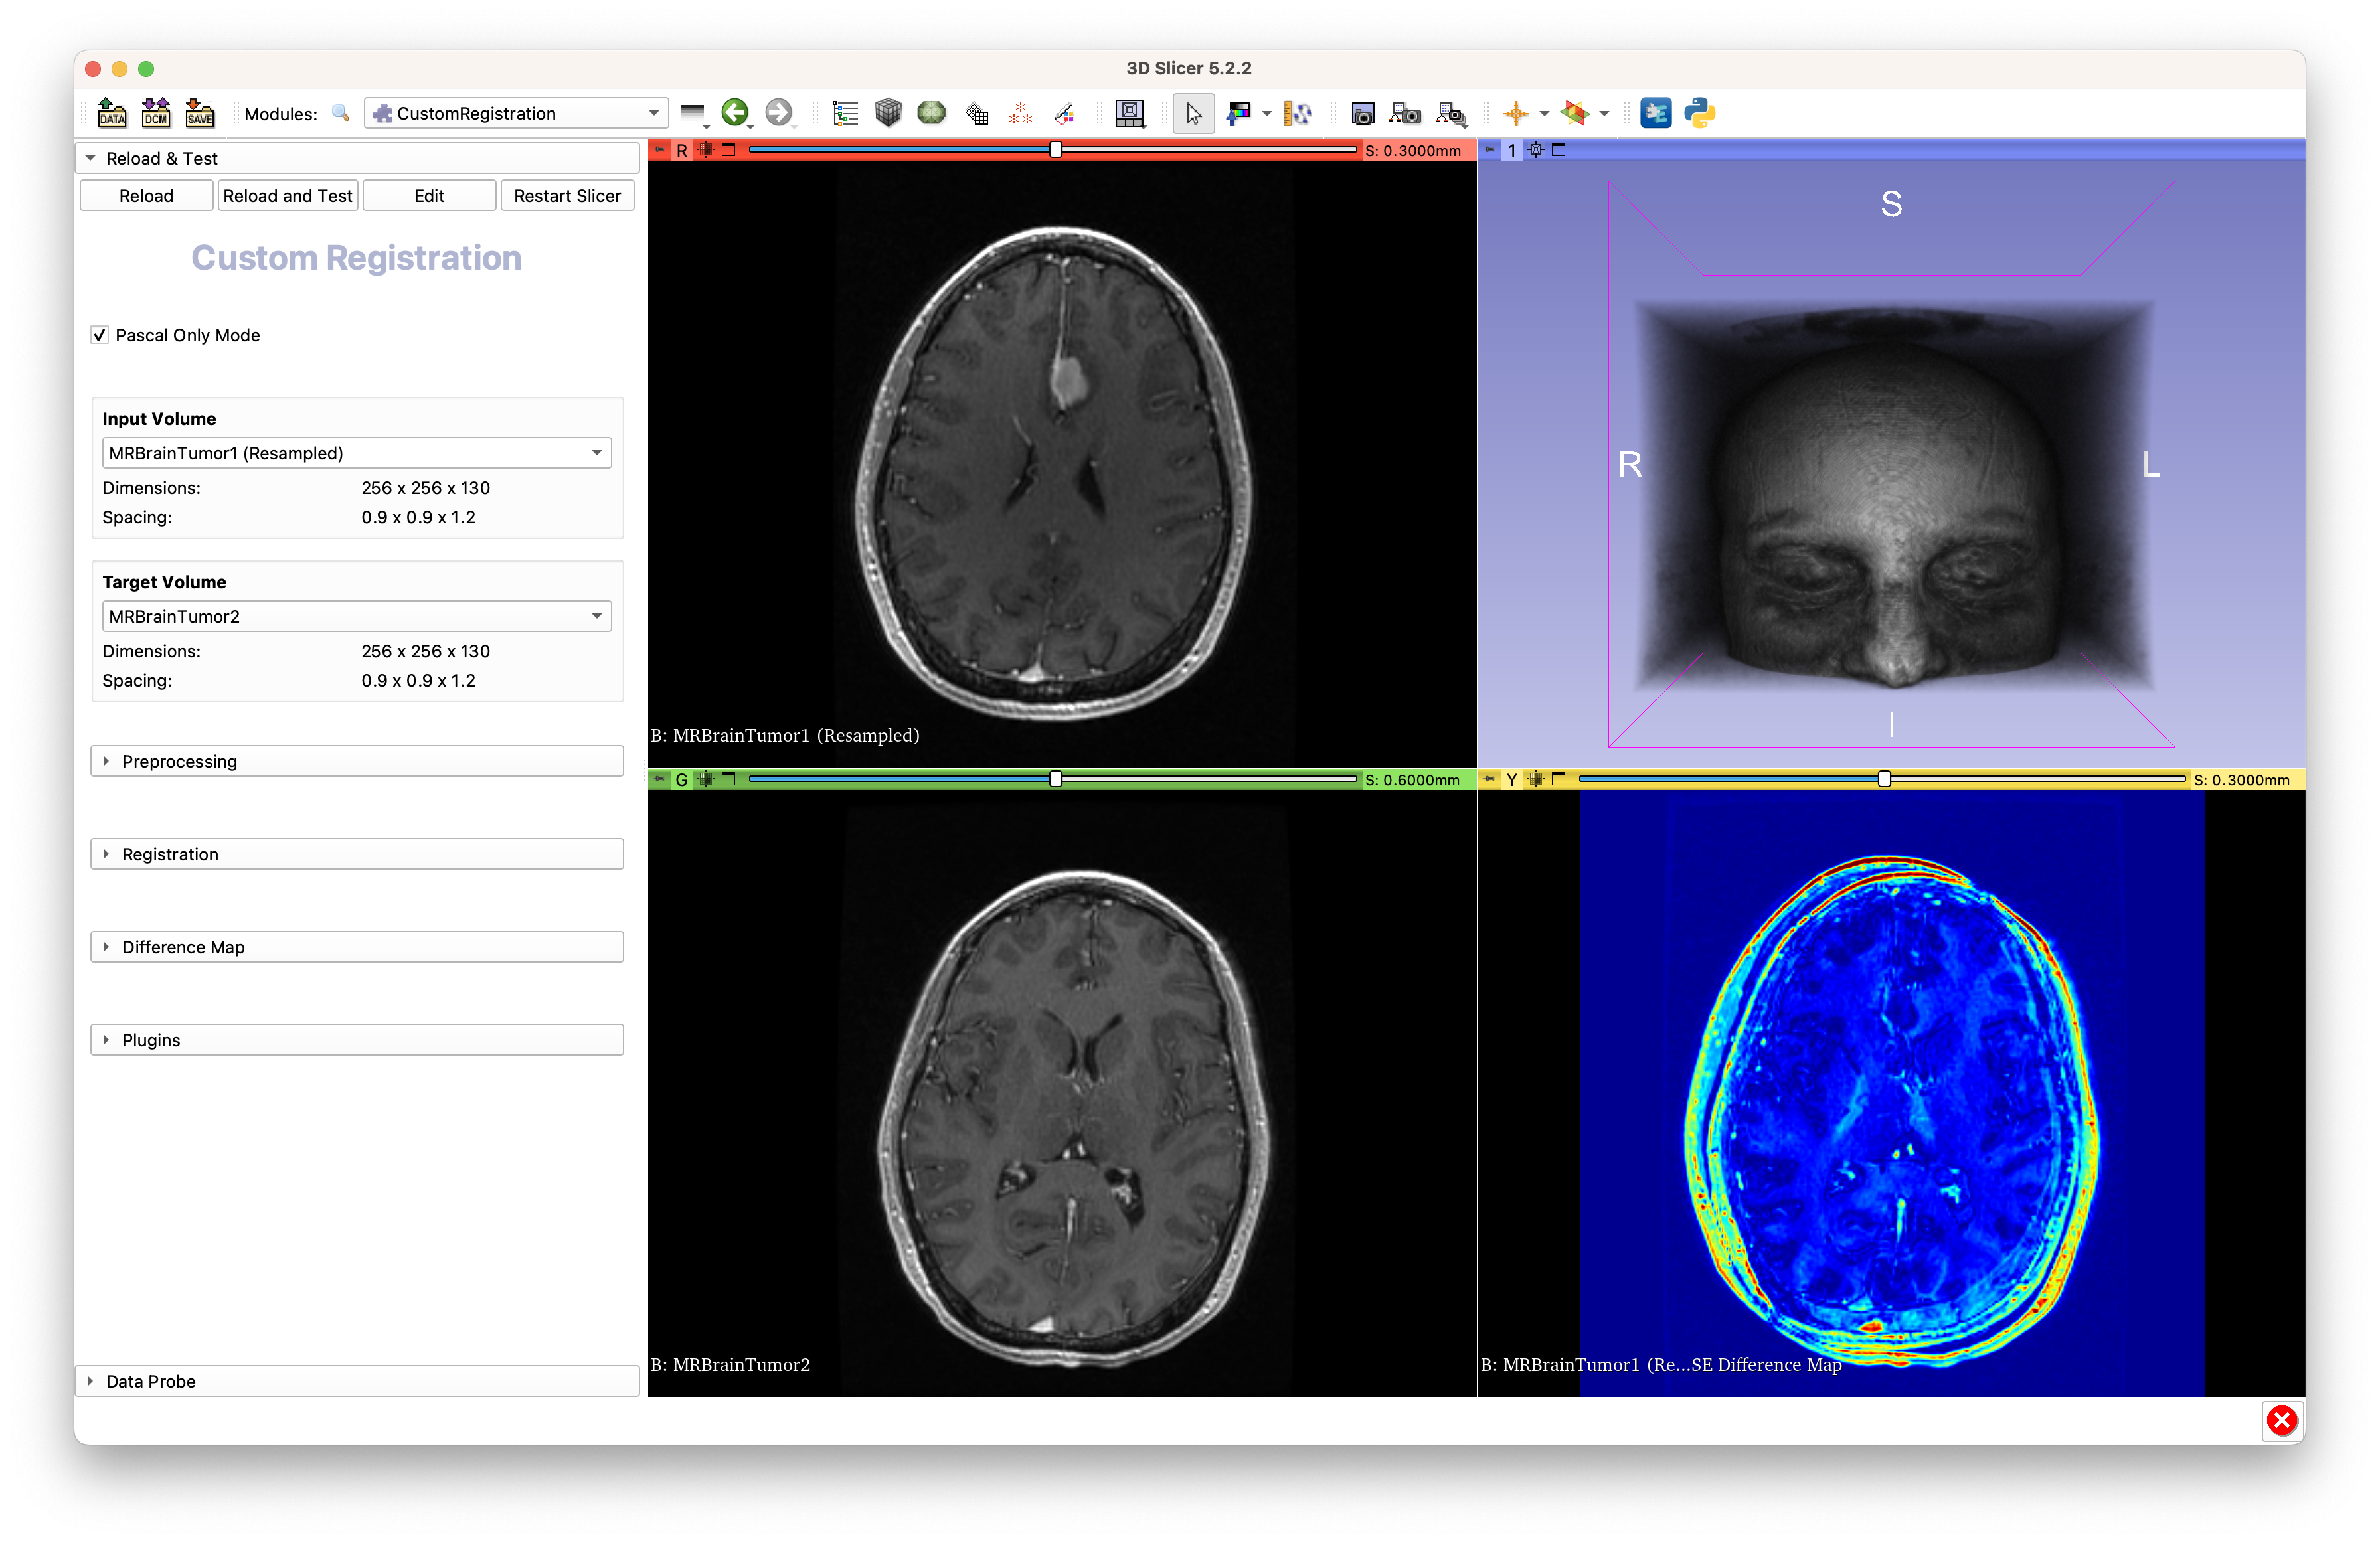
\includegraphics[width=\textwidth]{images/general-view.png}
                    \caption{Aperçu général du module d'extension basé sur la maquette (Figure~\ref{fig:ui-mock-up}), comprenant le panneau de traitements à gauche et les différentes vues à droite (en haut à gauche la vue 2D de l'image d'entrée, en haut à droite la vue 3D optionnelle du mode Pascal Only, en bas à gauche la vue 2D de l'image cible, en bas à droite la vue 2D de la carte de différence.}
                    \label{fig:general-view}
                \end{minipage}

                \bigskip\bigskip\bigskip

                \begin{minipage}{\textwidth}
                    \centering
                    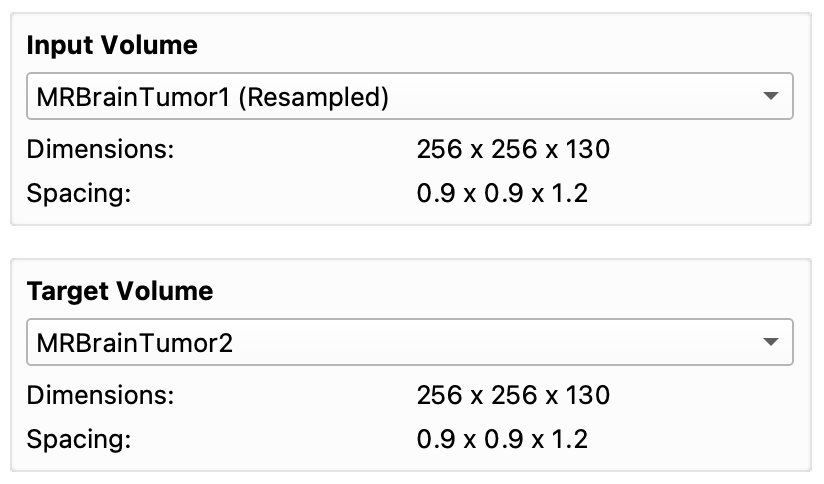
\includegraphics[width=0.5\textwidth]{images/input-target-ui.png}
                    \caption{Aperçu de l'UI du système de choix d'image d'entrée (Input Volume) et d'image cible (Target Volume) basé sur la maquette (Figure~\ref{fig:ui-mock-up}), comprenant les dimensions et la taille des voxels dans les trois dimensions des images.}
                    \label{fig:input-target-ui}
                \end{minipage}
            \end{figure}

            \bigskip

            Pour mettre en place le système d'images d'entrée/cible, deux séries de méthodes ont été implémentées~: l'une pour la gestion de l'image d'entrée, l'autre pour celle de l'image cible. Les deux séries sont dédiées aux mêmes tâches, mais appliquées aux deux cas bien distincts avec leurs propres particularités.

            \bigskip
            \method{setup\_<intput/target>\_volume}

            Méthode qui configure le système dédié à l'image d'entrée/cible, au même titre que \texttt{setup\_<feature>} vu précédemment. Elle est donc appelée par la méthode \texttt{setup} générale et se charge d'initialiser les données et de récupérer les éléments de l'UI. Concrètement, elle récupère les listes déroulantes de sélection d'image et y insère les actions sur les volumes disponibles (renommage et suppression). Elle lie ensuite les actions à leurs évènements respectifs (méthodes associées à la sélection, au renommage et à la suppression détaillées ci-dessous).

            \bigskip
            \method{reset\_<input/target>\_volume}

            Méthode qui rétablit l'état par défaut du système dédié à l'image d'entrée/cible, au même titre que \texttt{reset\_<feature>} vu précédemment. Ici, il suffit alors de désélectionner l'éventuelle image d'entrée/cible grâce à la méthode suivante.

            \bigskip
            \method{select\_<input/target>\_volume}

            Méthode qui sélectionne une image comme image d'entrée/cible par son identifiant dans la liste des images. Si l'identifiant est -1 (valeur par défaut), aucune image ne sera sélectionnée (il s'agit de l'état par défaut). Elle est appelée lorsque la liste déroulante change de valeur (c'est-à-dire que l'utilisateur change d'image sélectionnée), ainsi que par \texttt{reset\_<input/target>\_volume} (avec l'identifiant -1). La référence en mémoire de l'image d'entrée/cible est alors adaptée, et la méthode \texttt{update} générale est appelée afin de mettre à jour le module d'extension en fonction.

            \bigskip
            \method{rename\_<input/target>\_volume}

            Méthode qui gère l'évènement du renommage de l'image d'entrée/cible actuellement sélectionnée. Cet évènement est déclenché lorsque l'utilisateur choisi l'action de renommage depuis la liste déroulante (si une image est sélectionnée comme image d'entrée/cible). Le nom de l'image d'entrée/cible est alors modifié et le module d'extension actualisé.

            \bigskip
            \method{delete\_<input/target>\_volume}

            Méthode qui gère l'évènement du suppression de l'image d'entrée/cible actuellement sélectionnée. Cet évènement est déclenché lorsque l'utilisateur choisi l'action de suppression depuis la liste déroulante (si une image est sélectionnée comme image d'entrée/cible). L'image d'entrée/cible est alors supprimée de la scène, et ses références sont remises à \texttt{None}. Aucune image n'est alors sélectionnée.

            \bigskip

            Le système de vues a été mis en place en suivant la même architecture que les fonctionnalités (Section~\ref{subsubsec:feature-architecture}), à l'exception d'une méthode.

            \bigskip
            \method{setup\_view}

            Méthode qui configure le système de vues. Elle est appelée par la méthode \texttt{setup} générale. Elle récupère les vues afin de pouvoir les manipuler par la suite, puis les initialise grâce à la méthode suivante.

            \bigskip
            \method{reset\_view}

            Méthode qui rétablit l'état par défaut des vues. Elle est appelée par \texttt{setup\_view}, par la méthode \texttt{reset} générale et dès que nécessaire à travers le module d'extension. Elle désactive l'affichage de tous les volumes avant tout, puis met à jour la vue selon les données actuelles via la méthode suivante.

            \bigskip
            \method{update\_view}

            Méthode qui met à jour les vues en fonction de la scène actuelle, et des images sélectionnées comme images d'entrée et cible. Elle est appelée par la méthode \texttt{reset\_view}, par la méthode \texttt{update} générale et dès que nécessaire à travers le module d'extension. Elle utilise la méthode suivante pour afficher les images sélectionnées dans les vues appropriées.

            \bigskip
            \method{update\_specific\_view}

            Méthode qui, comme son nom l'indique, met à jour une vue spécifique dont l'identifiant est spécifié en paramètre, avec la référence d'une image, et éventuellement la référence d'un volume à afficher en transparence par dessus l'image choisie (\texttt{mask}).
        }
    }

    % Prétraitements
    {
        \bigskip
        \subsection{Prétraitements}
        \label{subsec:preprocessing-implementation}

        % Sélection de ROI
        {
            \subsubsection{Sélection de ROI}
            \label{subsubsec:roi-selection-preprocessing-implementation}

            La sélection de ROI est un outil n'affectant pas l'image directement. Il s'agit seulement de sélectionner une zone spécifique dans l'image contenant des informations pertinentes pour l'analyse ou le traitement ultérieur.

            La sélection de ROI peut être utilisée pour faciliter les traitements des images, en particulier le recalage, en identifiant les zones d'intérêt communes à plusieurs images. Une fois la ROI sélectionné, elle peut être utilisée comme référence pour le traitement/l'alignement des images, permettant d'assurer que les zones d'intérêt correspondent bien les unes aux autres dans toutes les images.

            \bigskip

            Suivant la \hyperref[us:preprocessing]{US I}, la sélection de ROI est implémentée grâce à la méthode du seuillage binaire. L'implémentation s'est donc faite en deux étapes.

            Une première méthode de la classe \texttt{Logic}, \texttt{create\_mask}, se charge d'effectuer une binarisation de l'image passée en paramètre au format \textit{VTK Volume}, grâce à une valeur de seuillage également passée en paramètre. L'image est tout d'abord convertie au format \textit{SimpleITK Image} afin que le seuillage puisse être effectué grâce à la méthode de \textit{SimpleITK} \texttt{BinaryThreshold}. La méthode \texttt{create\_mask} retourne alors la nouvelle image correspondant à cette binarisation, convertie au format \textit{VTK Volume}.

            Toujours dans la classe \texttt{Logic}, une deuxième méthode, \texttt{select\_roi}, prend en paramètre l'image sur laquelle la ROI doit être sélectionnée et la masque calculée par la première méthode, les deux au format \textit{VTK Volume}. Ils sont avant tout convertis au format \textit{SimpleITK Image}. La méthode se charge alors de récupérer la plus grande composante connexe du masque (l'image binarisée). Cette nouvelle version de l'image correspond alors à la ROI. Celle-ci est convertie au format \textit{VTK Volume} à nouveau afin de pouvoir être manipulée dans la scène de 3D~Slicer.

            \bigskip

            Il est possible de sélectionner une ROI sur une image simplement, ou bien en parallèle sur deux images, de la même manière sur l'interface dédiée. L'utilisateur doit avoir préalablement sélectionné une image comme image d'entrée et/ou une comme image cible via l'interface supérieure.

            Suivant la maquette établie lors de la conception (Figure~\ref{fig:roi-ui-mock-up}) et appliquant cette possibilité de sélection les ROI de deux images distinctes, dans la section \textit{ROI Selection}, deux curseurs coulissants (\textit{sliders}) sont présents pour permettre à l'utilisateur de choisir une valeur de seuillage sur chacune des images. Ces \textit{sliders} sont liés à la méthode \texttt{Logic.create\_mask} pour sauvegarder en mémoire les masques. Le bouton \textit{Select ROI} est lié à la méthode \texttt{Logic.select\_roi}.  Au clic sur le bouton \textit{Select ROI}. La ROI ainsi calculée est sauvegardée dans un dictionnaire liant les images et leur ROI, \texttt{volume\_roi\_map}. L'interface est représentée en Figure~\ref{fig:roi-selection-ui}.

            \begin{figure}[!ht]
                \centering
                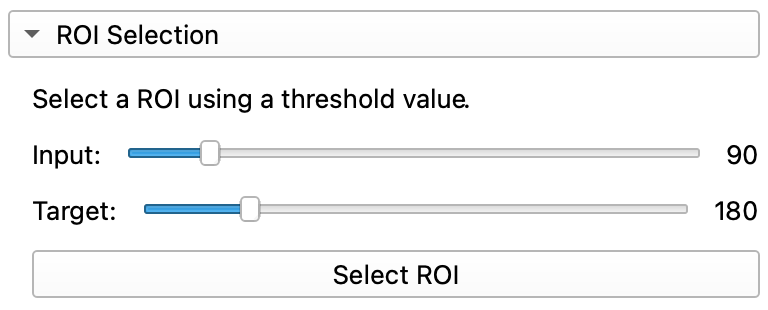
\includegraphics[width=0.5\textwidth]{images/roi-selection-ui.png}
                \caption{Aperçu de l'interface de sélection de ROI.}
                \label{fig:roi-selection-ui}
            \end{figure}

            % Prévisualisation et visualisation finale
            {
                \subsubsubsection{Prévisualisation et visualisation finale}

                Afin d'améliorer l'ergonomie de la fonctionnalité de sélection de ROI, nous avons intégré des options de prévisualisation et de visualisation. Elles permettent à l'utilisateur de visualiser la région de l'image désignée respectivement avant et après validation de la sélection. Ainsi, l'utilisateur peut ajuster le seuil pour choisir la région adéquate pour son application.

                \bigskip

                La prévisualisation est générée dans la méthode \texttt{preview\_roi\_selection} de la classe \texttt{Widget}.
                Cette méthode a l'avantage de gérer plusieurs variations. En effet, comme la sélection de la ROI peut être effectuée sur l'image d'entrée et/ou l'image cible, notre méthode offre trois options~: \texttt{"input"}, \texttt{"target"} ou \texttt{"all"} qui permettent de générer une prévisualisation adéquatement au cas voulu.

                L'approche adoptée pour illustrer la ROI consiste afficher sur la vue concernée le \textit{VTK Volume} en avant-plan transparent et d'attribuer la couleur rouge aux voxels lors de l'affichage, grâce à une \textit{Color Table} (classe \texttt{vtkMRMLColorTableNode}).

                La première étape du processus général est de supprimer le précédent affichage s'il existe.
                Ensuite, il convient de récupérer le seuil entré par l'utilisateur grâce au \texttt{slider} adéquat. À partir de celui-ci et de l'image sélectionnée comme entrée/cible, on peut récupérer le masque représentant la binarisation grâce à la méthode \texttt{Logic.create\_mask} mentionnée précédemment.
                Il convient de noter que l'intervalle des sliders qui permettent de choisir un seuil est configuré pour correspondre à la plage dynamique de l'image traitée afin d'éviter les erreurs de valeurs.
                Par la suite, le \textit{Display Node} (classe \texttt{vtkMRMLScalarVolumeDisplayNode}) --- permettant de paramétrer l'affichage de l'image --- est récupéré afin de lui assigner la \textit{Color Table} définie au préalable. Il suffit ensuite d'ajouter le \textit{VTK Volume} représentant la ROI à la scène.
                Enfin, il convient d'afficher le masque par-dessus l'image traitée (\textit{foreground}), en transparence (50\%), afin de pouvoir visualiser convenablement la zone sélectionnée (voir Figure~\ref{fig:roi-selection-preview}).

                \bigskip

                Quant à la visualisation, elle se passe dans la méthode \texttt{display\_roi} de la classe \texttt{Widget}.
                Elle fonctionne exactement de la même manière que \texttt{preview\_roi\_selection}. La différence réside seulement dans la couleur d'affichage qui est cette fois verte (voir Figure~\ref{fig:roi-selection-view}), et le \textit{VTK Volume} utilisé qui n'est pas la binarisation sauvegardée en mémoire, mais la ROI stockée dans le dictionnaire \texttt{volume\_roi\_map}.

                \begin{figure}[!ht]
                    \centering
                    \begin{minipage}[t]{0.45\textwidth}
                        \centering
                        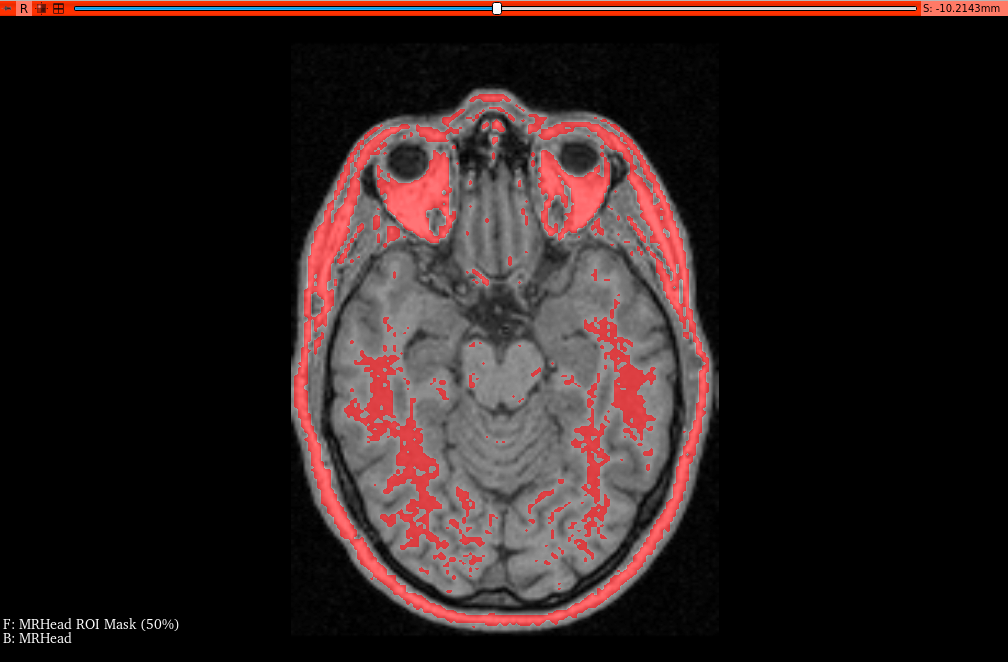
\includegraphics[width=\textwidth]{images/roi-selection-preview.png}
                        \caption{Exemple de prévisualisation de sélection de ROI (avec un seuil \texttt{Threshold=90}) sur une IRM d'une tête (échantillon disponible sur 3D Slicer), depuis un angle axial.}
                        \label{fig:roi-selection-preview}
                    \end{minipage}
                    \hfill
                    \begin{minipage}[t]{0.45\textwidth}
                        \centering
                        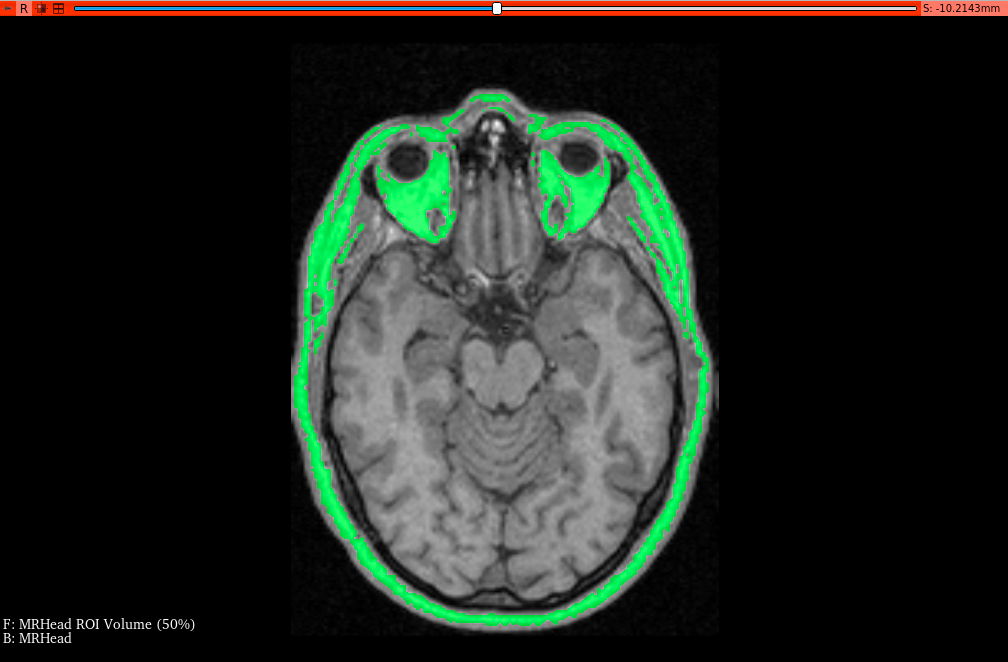
\includegraphics[width=\textwidth]{images/roi-selection-view.png}
                        \caption{Exemple de visualisation de sélection de ROI suite à la sélection de la Figure~\ref{fig:roi-selection-preview}.}
                        \label{fig:roi-selection-view}
                    \end{minipage}
                \end{figure}

                \bigskip

                La mise à jour de la prévisualisation et de la visualisation finale se fait dans une seule et même méthode \texttt{Widget.update\_roi\_selection}. Elle est sollicitée chaque fois que l'utilisateur bouge un \textit{slider}.

                De surcroît, puisqu'une vue sur 3D~Slicer ne peut afficher que deux images à la fois, elle s'occupe d'afficher la prévisualisation si le panneau de la sélection de ROI est ouvert, la visualisation finale sinon (si elle existe).

                \newpage
            }

            % Limitations
            {
                \subsubsubsection{Limitations}

                % Factorisation de preview et display_roi comme perspective ?

                La sélection de ROI telle qu'implémentée présente cependant plusieurs limitations.

                \bigskip

                Tout d'abord un bug est connu mais sa réparation n'a pas pu se faire par manque de temps. En effet, si l'on tente de faire une double sélection de ROI (images d'entrée/cible en parallèle) mais sur la même image, le processus ne s'arrête pas car il n'y a pas d'erreurs, mais les références en mémoire sont erronées pour l'une des sélections (il n'y a qu'une seule ROI associée à l'image, alors qu'il y a deux visualisations avec des références distinctes). Le résultat est une visualisation correcte, mais une autre affichant le mauvais volume en avant-plan transparent, comme on peut le voir en Figure~\ref{fig:roi-selection-bug}.

                \begin{figure}[!ht]
                    \centering
                    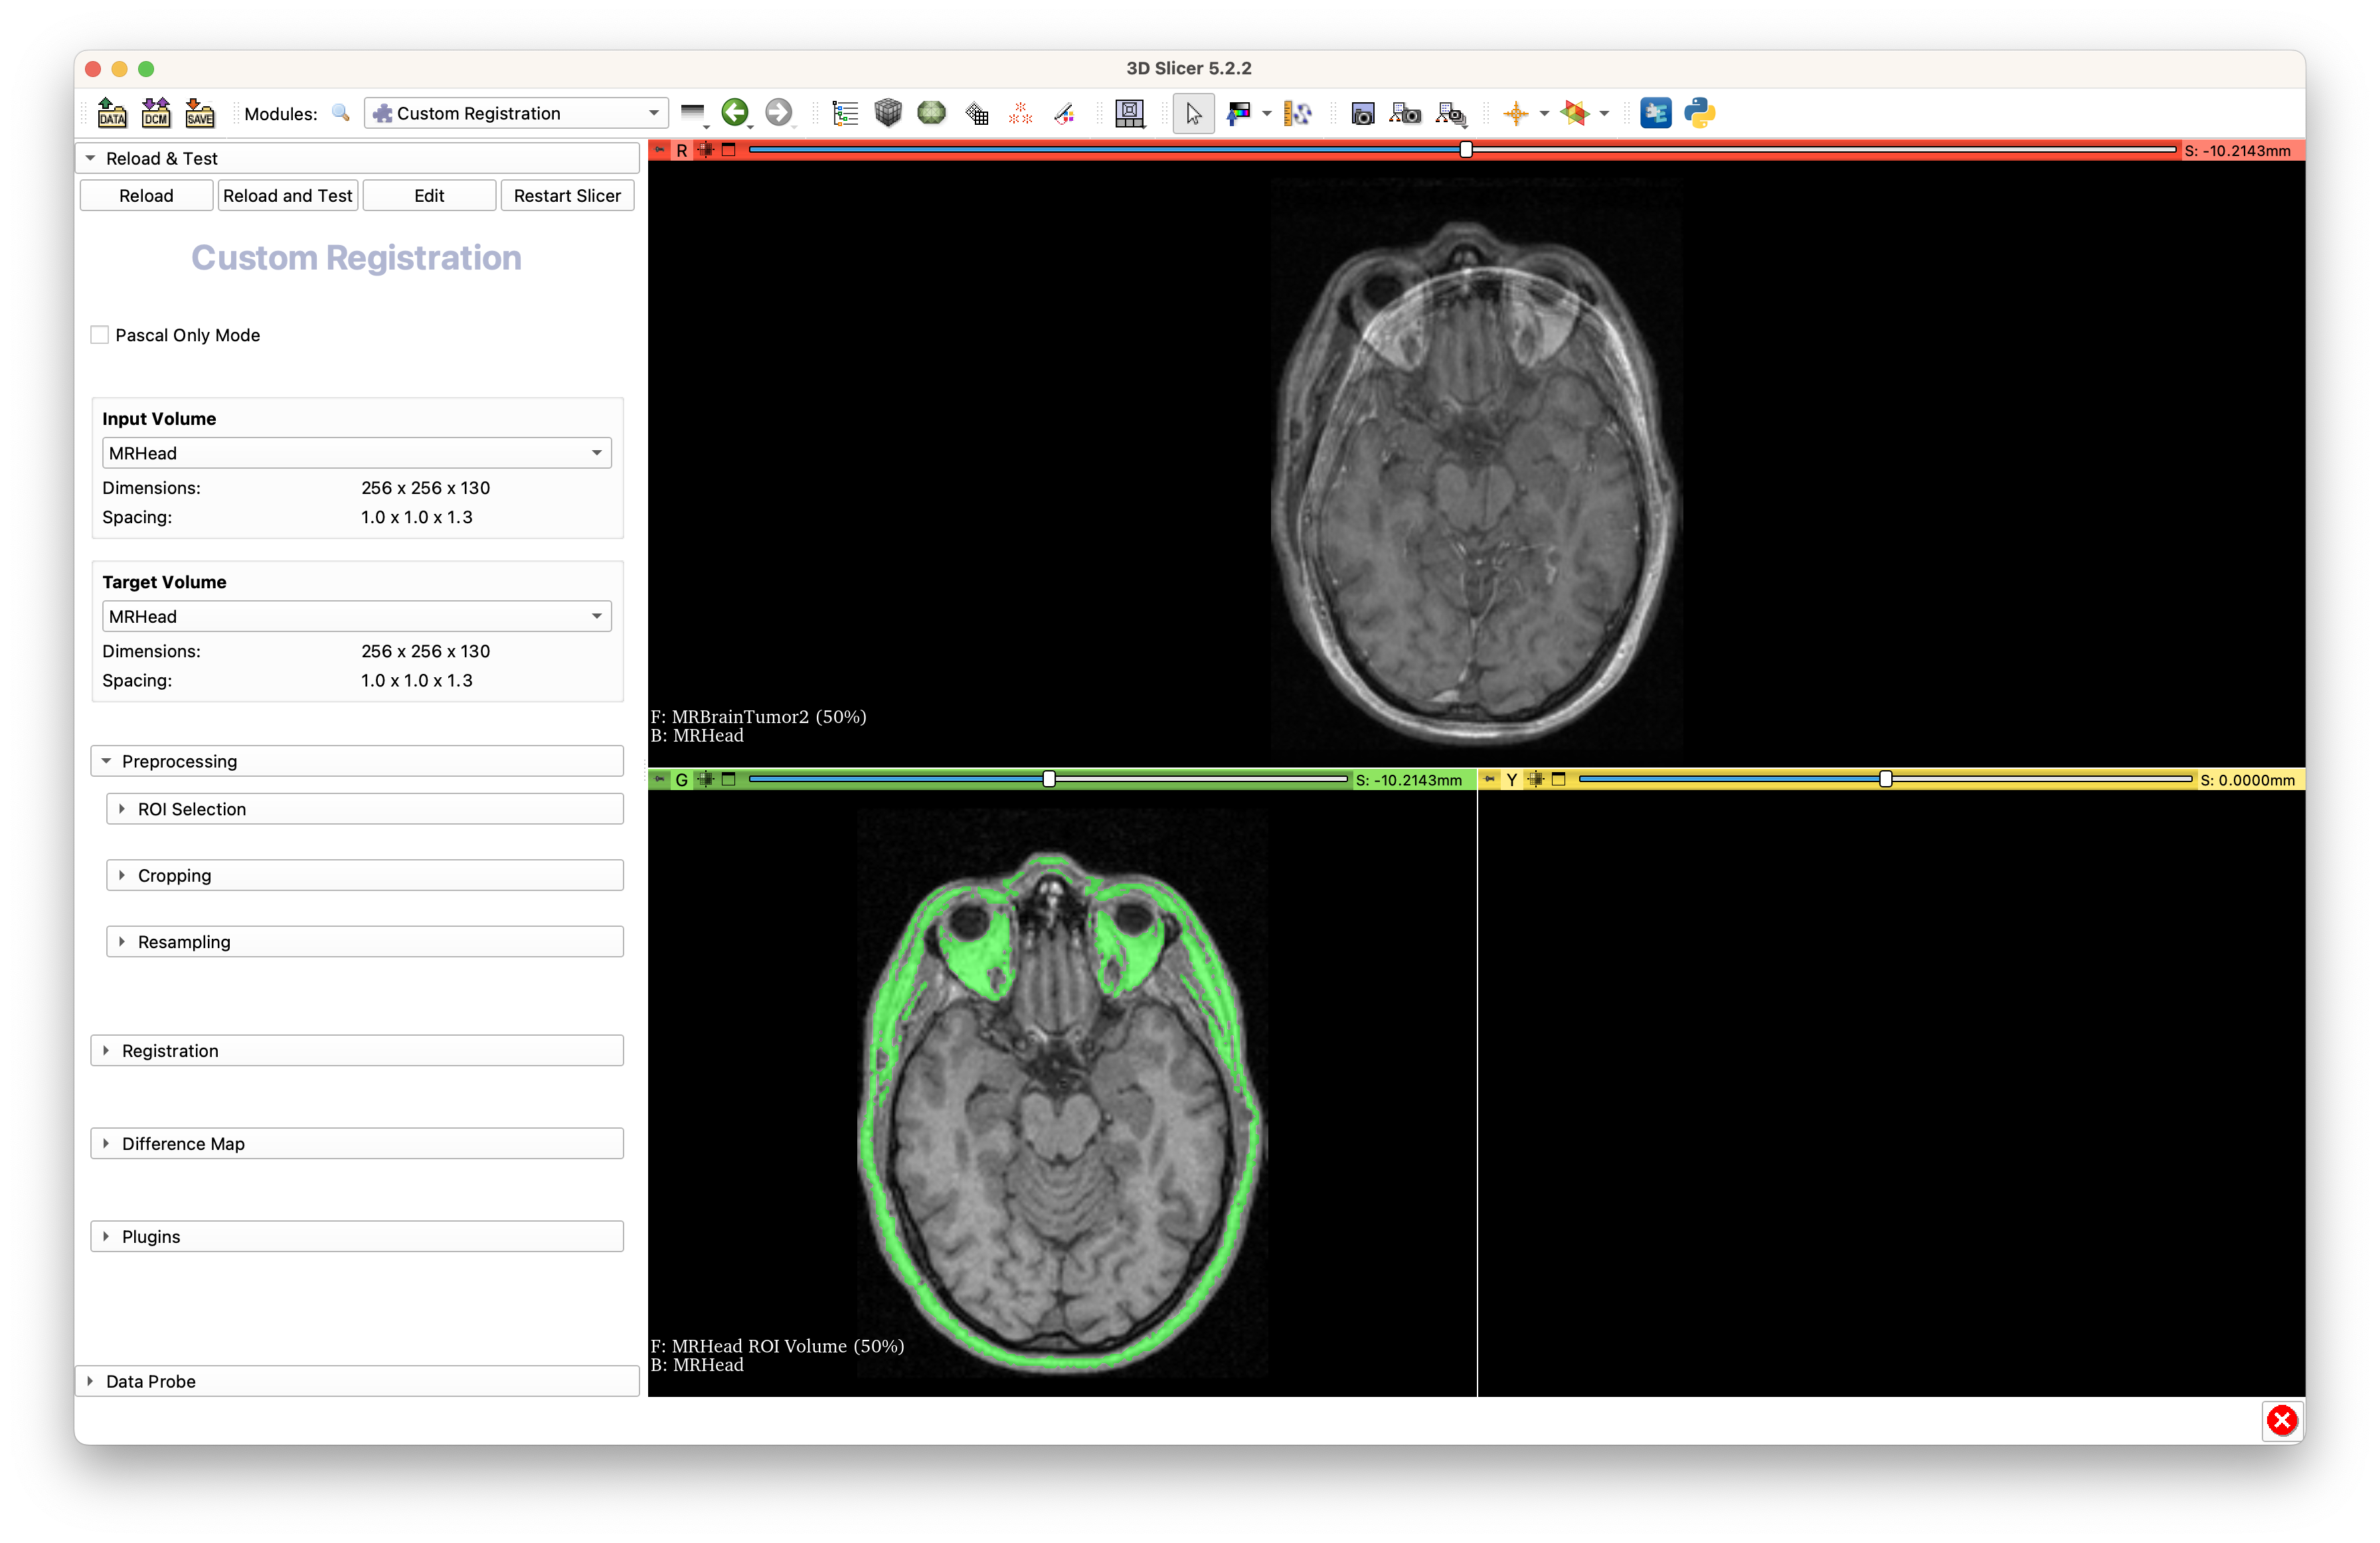
\includegraphics[width=\textwidth]{images/roi-selection-bug.png}
                    \caption{Bug de la double sélection de ROI en parallèle sur la même image.}
                    \label{fig:roi-selection-bug}
                \end{figure}

                \bigskip

                En outre, cette méthode de sélection de ROI est limitée dans son aptitude à sélectionner précisément une ROI. En effet, l'utilisateur n'a pas de contrôle sur la ROI sélectionnée, seulement sur le seuillage préalable. Or, il pourrait voudrait choisir un tissu unique en particulier par exemple. Cette méthode permet cependant une simplicité et rapidité d'utilisation.

                \bigskip

                Enfin, au niveau du code, il serait pertinent de simplifier les appels aux méthodes en factorisant \texttt{Widget.preview\_roi} et \texttt{Widget.display\_roi} qui se chargent toutes les deux d'afficher des volumes en avant-plan transparent, mais dans deux cas différents.
            }
        }

        % Rognage
        {
            \subsubsection{Rognage}
            \label{subsubsec:cropping-preprocessing-implementation}

            % Introduction
            {
                Le rognage est une opération de traitement d'image couramment utilisée pour découper une image en supprimant les parties inutiles, telles que les bords noirs, les zones de fond ou les parties qui ne sont pas pertinentes pour l'analyse.

                Cette opération est notamment utile en amont du recalage, afin de réduire la taille de l'image et de faciliter le traitement, tout en conservant les zones d'intérêt pour l'analyse. En éliminant les parties inutiles de l'image, le rognage peut améliorer la précision du recalage en réduisant les artefacts dus aux zones inutiles ou incohérentes de l'image. Le rognage peut également aider à minimiser les erreurs de recalage en réduisant les variations dans les régions environnantes des zones d'intérêt. En outre, la réduction de la taille de l'image peut également améliorer les performances du recalage en réduisant le temps de calcul et la consommation de mémoire.
            }

            % Rognage manuel
            {
                \bigskip
                \subsubsubsection{Rognage manuel}

                L'implémentation de l'algorithme de rognage manuel a été réalisée dans la méthode \texttt{crop} de la classe
                \\ \texttt{Logic}.
                Cette méthode requiert trois paramètres en entrée~: une image 3D au format \textit{VTK Volume} ainsi que deux tableaux de taille 3, décrivant les positions de début et de fin de l'image résultante dans le repère de l'image d'entrée.

                Pour commencer, l'image d'entrée est convertie en image \textit{SimpleITK}.
                Puis pour procéder au rognage, la classe \texttt{CropImageFilter} de la bibliothèque \textit{SimpleITK} est utilisée. Cette classe permet de créer un filtre en spécifiant les marges à enlever depuis le début et la fin des bords de l'image à rogner.
                Ensuite, la méthode \texttt{Execute} permet d'extraire une région de l'image 3D en fonction de ces paramètres. Puis on attribue à l'image rognée l'origine, l'espacement et la matrice de direction de l'image d'entrée afin que les deux images conservent les mêmes propriétés.
                Finalement, l'image 3D rognée est convertie au format \textit{VTK Volume} avant d'être retournée en tant que résultat final.

                \bigskip

                La gestion de ce traitement se fait dans la méthode \texttt{manual\_crop} de la classe \texttt{Widget}, qui est appelée lorsque l'utilisateur clique sur le bouton \textit{Crop}. Son rôle est principalement de sauvegarder l'image rognée en l'ajoutant à la liste des images 3D de la scène, puisqu'on verra par la suite que l'image rognée existe déjà avant que l'utilisateur ne clique sur le bouton \textit{Crop} (voir paragraphe \hyperref[subsubsubsec:cropping-preview]{prévisualisation}).

                En outre, elle se charge de gérer les erreurs de paramètres. Si l'utilisateur entre des paramètres invalides (une position de début supérieure ou égale à la position de fin) et confirme le traitement avec le bouton \textit{Crop}, une fenêtre avec un message d'erreur apparaîtra.
            }

            % Rognage automatique
            {
                \bigskip
                \subsubsubsection{Rognage automatique}
                \label{subsubsubsec:automatic-cropping}

                Le principe du rognage automatique est d'utiliser une ROI sélectionnée en amont pour définir une première zone à rogner, et d'ajouter une marge autour de celle-ci. Cette marge supplémentaire permet de tenir compte de certaines imperfections dans la sélection de la ROI, tout en garantissant que l'ensemble de l'objet d'intérêt soit bien présent dans l'image finale.

                \bigskip

                De la même manière que pour le rognage manuel, l'implémentation de l'algorithme de rognage automatique se fait dans la méthode \texttt{automatic\_crop} de la classe \texttt{Logic}.

                À la différence de la méthode \texttt{manual\_crop}, elle nécessite en entrée deux images 3D au format \textit{VTK Volume}~: l'image à rogner et l'image représentant la ROI grâce à des valeurs binaires. Elle demande également un tableau de taille 3 décrivant la taille des marges à ajouter autour de la boîte englobante de la ROI.
                Par la suite, elle récupère la boîte englobante de la ROI, (à ne pas confondre avec la boîte englobante de l'image représentant la ROI) avant d'y ajouter les marges.
                Pour finir, la méthode \texttt{crop} de la classe \texttt{Logic} génère l'image 3D rognée finale. Cette image est retournée avec sa boîte englobante (dans le repère de l'image d'entrée) à l'aide d'un tuple.

                \bigskip

                Toujours en suivant le même schéma que pour le rognage manuel, nous avons implémenté une méthode \texttt{automatic\_crop} dans la classe \texttt{Widget} qui est exécutée dès lors que l'utilisateur clique sur le bouton \textit{Automatic Crop}.

                Elle s'occupe donc, de la même façon, de charger dans la scène l'image rognée, générée en amont dans la méthode \texttt{preview\_automatic\_crop} (voir paragraphe \hyperref[subsubsubsec:cropping-preview]{prévisualisation}).

                Elle gère également les erreurs de paramètres (marges dépassant les limites de l'image d'entrée) entrés par l'utilisateur, en affichant une fenêtre avec un message d'erreur.

                Notons que pour utiliser ce mode de rognage, l'utilisateur doit avoir sélectionné une ROI au préalable. Autrement, une fenêtre de message d'erreur s'affichera pour lui signaler de le faire.
            }

            % Paramétrage
            {
                \bigskip
                \subsubsubsection{Paramétrage}

                En premier lieu, afin de choisir un mode de rognage, nous proposons des boutons d'option \textit{Manual} et \textit{Automatic} (voir Figures~\ref{fig:manual-cropping-ui} et~\ref{fig:automatic-cropping-ui}). Pour plus de lisibilité, seule l'UI du mode sélectionné est affichés.

                \bigskip

                Pour rogner une image manuellement, l'utilisateur a à sa disposition des zones de saisie numérique à incrémentation (voir Figure~\ref{fig:manual-cropping-ui}) qui lui permettent d'entrer les bords de l'image rognée souhaitée, (positions de début et de fin, qu'on appellera par la suite boîte englobante) dans le repère de l'image d'entrée. Par ailleurs, ces zones de saisie sont paramétrées de telle sorte qu'on ne puisse pas entrer des positions en dehors des dimensions de l'image d'entrée.

                \bigskip

                Pour rogner une image automatiquement, l'utilisateur dispose également de zones de saisie numérique à incrémentation (Figure~\ref{fig:automatic-cropping-ui}). Celles-ci permettent d'entrer la taille des marges à ajouter autour de la sélection de ROI. Contrairement à celles du rognage manuel, les valeurs maximales des zones de saisie ne sont pas définies en fonction des limites maximales autorisées (le minimum est paramétré à 0 par défaut, ce qui nous convient). Cette situation est prise en compte ultérieurement lors de l'opération de sauvegarde (voir paragraphe \hyperref[subsubsubsec:automatic-cropping]{Rognage automatique}).

                \begin{figure}[!ht]
                \centering
                \begin{minipage}[t]{0.45\textwidth}
                    \centering
                    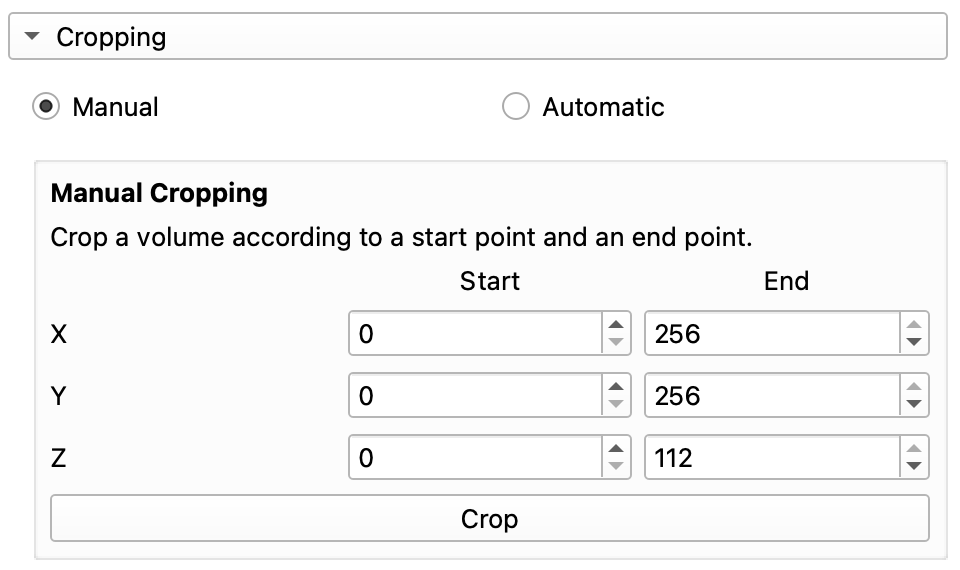
\includegraphics[width=\textwidth]{images/manual-cropping-ui.png}
                    \caption{Aperçu de l'UI de rognage manuel.}
                    \label{fig:manual-cropping-ui}
                \end{minipage}
                \hfill
                \begin{minipage}[t]{0.45\textwidth}
                    \centering
                    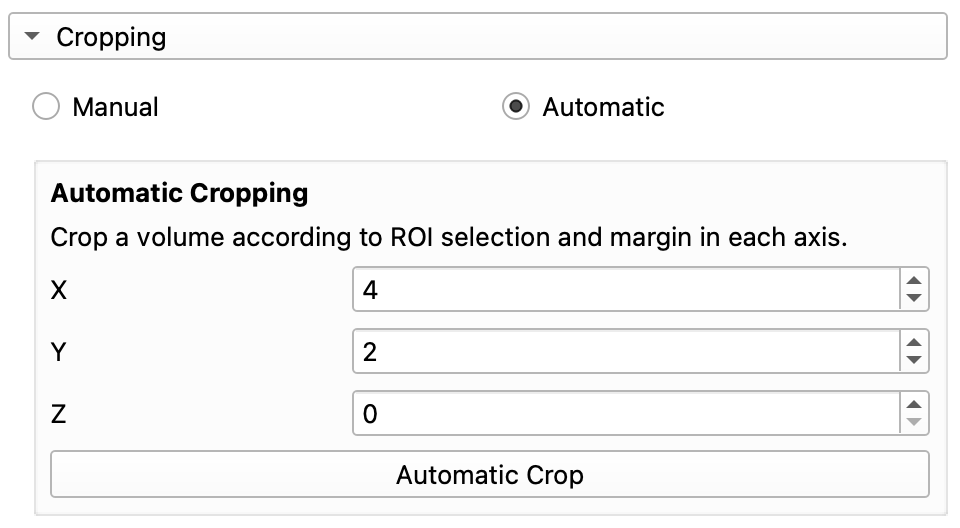
\includegraphics[width=\textwidth]{images/automatic-cropping-ui.png}
                    \caption{Aperçu de l'UI de rognage automatique.}
                    \label{fig:automatic-cropping-ui}
                \end{minipage}
                \end{figure}
            }

            % prévisualisation
            {
                \bigskip
                \subsubsubsection{Prévisualisation}
                \label{subsubsubsec:cropping-preview}

                Dans l'optique de faciliter l'utilisation du rognage, nous avons ajouté une fonctionnalité de prévisualisation. Cette fonctionnalité permet à l'utilisateur de visualiser la région de l'image qui sera rognée avant d'exécuter le rognage. Ainsi, l'utilisateur peut mieux sélectionner la région souhaitée pour son application, en évitant les erreurs potentielles de rognage.

                \bigskip

                Ce processus a lieu, de manière similaire, dans les deux méthodes dédiées de la classe \texttt{Widget}, \texttt{preview\_manual\_cropping} et \texttt{preview\_automatic\_cropping}.

                L'idée est de créer un objet \textit{ROI Markup Node} (de type \texttt{vtkMRMLMarkupsROINode}) qui représente en fait une boîte semi-transparente, de couleur rouge par défaut (voir Figure~\ref{fig:cropping-preview}). Le fait que ce soit une boîte et non un rectangle (autrement dit un objet 3D et non un objet 2D) permet à l'utilisateur de prévisualiser la zone à rogner sur toutes les \textit{slices} et sous les trois vues proposées par 3D~Slicer (axiale, sagittale et coronale).

                \begin{figure}[!ht]
                    \centering
                    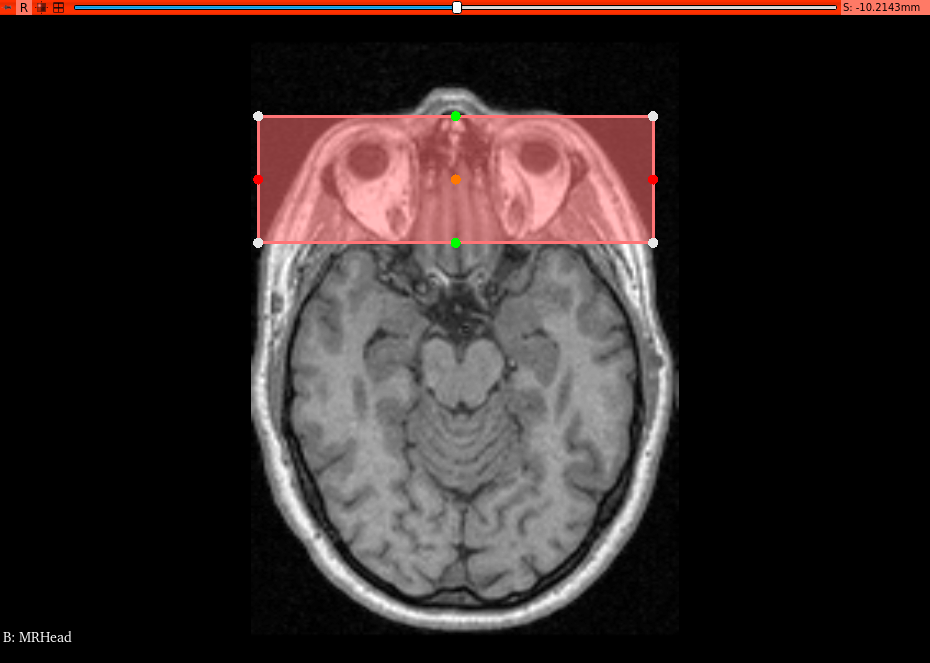
\includegraphics[width=0.5\textwidth]{images/cropping_preview.png}
                    \caption{Exemple de prévisualisation du rognage manuel (avec les paramètres \texttt{Start=(40, 0, 10)} et \texttt{End=(90, 200, 130)}) sur une IRM d'une tête (échantillon disponible sur 3D Slicer), depuis un angle axial.}
                    \label{fig:cropping-preview}
                \end{figure}

                Le procédé consiste dans un premier temps de supprimer le \textit{ROI Markup Node} précédent s'il existe et de calculer le nouveau en appelant \texttt{preview\_manual\_cropping} (ou \texttt{preview\_automatic\_cropping}).
                Puis, à effectuer le rognage sur l'image choisie par l'utilisateur (\textit{Input Volume}, Figure~\ref{fig:input-target-ui}) avec la méthode \texttt{Logic.crop} (ou \texttt{Logic.automatic\_crop}), à partir des paramètres entrés par l'utilisateur.
                Si les paramètres sont invalides, il n'y aura aucun message d'erreur mais la prévisualisation ne s'affichera pas.
                S'il n'y a pas d'erreur, la boîte englobante de l'image 3D rognée dans le repère global est ensuite récupérée. De la même manière que lorsqu'on utilise la méthode utilitaire \texttt{transfer\_volume\_metadata} après avoir créé le \textit{VTK Volume} pour l'image rognée, on affecte au \textit{ROI Markup Node} les mêmes propriétés que l'image originale. Cela permet de bien dimensionner la boîte de prévisualisation, et de la transformer (du repère local de l'image d'entrée) vers le repère global. Contrairement à un \textit{VTK Volume}, on ne peut pas assigner directement les méta-données à un \textit{ROI Markup Node}. C'est pourquoi nous sommes contraints d'appliquer les transformations directement sur la boîte englobante récupérée précédemment.

                \bigskip

                La gestion de la prévisualisation se fait dans la méthode \texttt{update\_cropping} (de la classe \texttt{Widget}), indépendemment du mode de rognage choisi. Elle est appelée dès lors que l'utilisateur modifie un paramètre.

                Dans la même idée que pour la sélection de ROI (voir Section~\ref{subsubsec:roi-selection-preprocessing-implementation}), elle gère l'affichage du \textit{ROI Markup Node}. Lorsque l'utilisateur ferme le panneau dépliant du rognage, la prévisualisation associée reste en mémoire et demeure cachée. Toutefois, cette dernière réapparaît lorsque le panneau est ouvert à nouveau.
            }

            % Limitations
            {
                \bigskip
                \subsubsubsection{Limitations}

                Finalement, notre implémentation comporte des limites au niveau de la prévisualisation. En effet, le calcul du \textit{ROI Markup Node} n'est pas optimisé. Même si l'utilisateur ne valide pas le rognage, il est quand même appliqué sur l'image 3D afin de générer la prévisualisation, et ce à chaque fois qu'un paramètre est modifié. Notons tout de même que l'affichage reste en temps réel et ne nuit pas à l'utilisation de la fonctionnalité.

                De plus, les points de contrôle du \textit{ROI Markup Node} ne sont pas interactifs, ce qui aurait pu être pratique pour que l'utilisateur puisse ajuster manuellement la zone à rogner.
            }
        }

        % rééchantillonage
        {
            \subsubsection{Rééchantillonnage}
            \label{subsubsec:resampling-preprocessing-implementation}

            Le rééchantillonnage est une opération de traitement d'image permettant de modifier la résolution spatiale d'une image en modifiant la taille des voxels ainsi que les dimensions de l'image.

            En général, le rééchantillonnage est nécessaire lorsque l'on souhaite aligner plusieurs images 3D acquises avec différents protocoles d'imagerie, ou lorsque l'on souhaite comparer des images avec différentes résolutions spatiales. Il s'agit donc d'une opération nécessaire avant un recalage ou un calcul de carte de différence.

            Ce rééchantillonnage peut se faire par interpolation, c'est-à-dire en utilisant des méthodes mathématiques pour estimer les valeurs des nouveaux voxels manquantes entre les voxels existants.

            \bigskip

            Dans notre optique de traitement minimal suivant la \hyperref[us:preprocessing]{US I}, le rééchantillonnage est conçu de sorte de rééchantillonner l'image d'entrée en fonction de l'image cible.

            L'interface dédiée est très simple et suit complètement la maquette prévue lors de la conception (Figure~\ref{fig:resampling-ui-mock-up}). Cette interface est représentée par la Figure~\ref{fig:resampling-ui}.

            \begin{figure}[!ht]
                \centering
                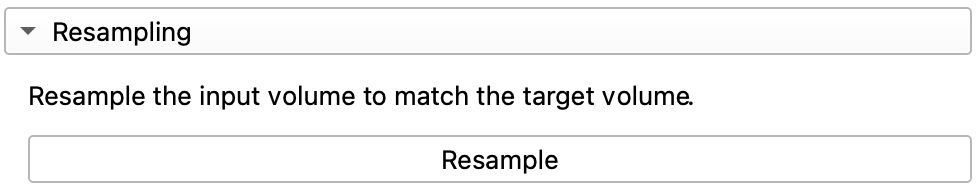
\includegraphics[width=0.5\textwidth]{images/resampling-ui.png}
                \caption{Aperçu de l'UI de rééchantillonnage.}
                \label{fig:resampling-ui}
            \end{figure}

            \bigskip

            L'implémentation de l'algorithme de rééchantillonage se fait dans la méthode \texttt{Logic.resample}. Cette méthode prend en paramètres les images d'entrée et cible au format \textit{VTK Volume}.

            Le volume rééchantillonné est créé grâce à la méthode \texttt{Resample} de la bibliothèque \texttt{SimpleITK}, en utilisant l'interpolateur par défaut. Les deux volumes \textit{VTK} sont convertis en image \textit{SimpleITK} au préalable, et l'image \textit{SimpleITK} sortie de est convertie au format \textit{VTK}, et les méta-données de ce type d'objets sont mises à jours pour correspondre à celles de l'objet \textit{SimpleITK}. Le volume rééchantillonné est alors retourné, l'algorithme étant terminé.

            \bigskip

            Dans la méthode \texttt{Widget.resample}, appelée lors du clic sur le bouton \textit{Resample}, se charge d'appeler \texttt{Logic.resample} avec les images d'entrée et cible sélectionnées par l'utilisateur, et d'ajouter l'image résultante à la scène de 3D~Slicer.
        }
    }

    % Recalage
    {
        \bigskip
        \subsection{Recalage}
        \label{subsec:registration-implementation}

        D'après \cite{registration}, “le recalage en imagerie médicale est une technique qui permet de superposer des images provenant de sources différentes ou de moments différents, afin de faciliter leur analyse ou leur interprétation”. C'est un outil
        essentiel pour surveiller l'évolution des patients, et rendre un diagnostique plus complet. Nous nous concentrons sur trois types de recalage.

        \begin{itemize}
            \item \textbf{Rigide} Suppose que les images sont liées par une rotation et une translation. Il préserve la forme et la taille des objets dans les images. Il contient 6 degrés de liberté.
            \item \textbf{Affine} Permet la mise à l'échelle et le cisaillement des images en plus de la rotation et de la translation. Il préserve les lignes parallèles, mais pas les angles ni les distances. Il contient 10 degrés de liberté.
            \item \textbf{Non-rigide} Permet de gérer les déformations locales des images qui ne sont pas prises en compte par les transformations rigides ou affines.
        \end{itemize}

        \bigskip

        L'objectif est d'intégrer au sein d'une même interface divers algorithmes de recalage disponibles sur deux bibliothèques principalement~: SimpleITk et Elastix. L'attente principale avec cette demande est l'accès aux outils de recalage, la comparaison de ces outils et de leur résultat. Cette comparaison pourra être effectué in fine avec des algorithmes de recalages personnalisés directement implémentables par l'utilisateur.

        \subsubsection{Implémentation logicielle}
        \label{subsubsec:softwaréregistration-implementation}

        L'implémentation de l'algorithme de recalage a été réalisée dans la méthode \texttt{register} de la classe \texttt{Logic}. Cette méthode se sert des images d'entrée et cible sélectionnées par l'utilisateur, c'est-à-dire l'image à recaler et l'image de référence (fixe).

        Une vérification des paramètres utilisateur est d'abord effectuée à l'entrée de la méthode. Selon le type de recalage adopté (SimpleITK, Elastix), la suite s'effectue via \texttt{custom\_script\_registration} ou \texttt{elastix\_registration}.

        \bigskip
        \subsubsubsection{Méthode custom\_script\_registration}

        Il s'agit d'une méthode auxiliaire utile à l'exécution d'un script python externe en tâche de fond via l'extension Slicer Parallel Processing. Deux scripts Python sont livrés avec notre extension~: \texttt{Rigid.py} et \texttt{NonRigid.py}. Tous deux intègrent des méthodes de recalage avec en entrées une image à recaler, une image fixe, et un dictionnaire propre à notre implémentation. Ce dictionnaire contient les paramètres pour chaque élément lié au recalage.

        \texttt{Rigid.py} agrège les types de recalages rigide et affine. Des méthodes utilitaires implémentées dans le fichier \texttt{Utilities.py} aident à la création de l'objet SimpleITK \texttt{ImageRegistrationMethod}, à l'aide du dictionnaire d'entrée, c'est cet objet qui se charge du recalage, via la méthode \texttt{Execute}. Les recalages de chaque fichier renvoient un objet \texttt{Transform}, celui-ci étant transformé en image avant d'être récupéré dans le module principal.

        \texttt{NonRigid.py} regroupe les recalages B-Spline et Demons dit non rigides.

        \bigskip
        \subsubsubsection{Méthode elastix\_registration}

        Cette méthode fait appel à \texttt{Elastix Logic}, un objet tiré de l'extension Slicer Elastix. La méthode de recalage \texttt{RegisterVolumes} prend en paramètres l'image fixe, l'image à recaler, un \textit{preset} de Slicer Elastix sélectionné au préalable, et un volume de sortie. Slicer Elastix n'est pas paramétrable par l'utilisateur autrement qu'avec les presets. Slicer Elastix est un choix d'intégration du client.

        \bigskip

        Le lancement d'un recalage exécute soit un script Python en tâche de fond, soit Slicer Elastix en tâche de fond. Lorsque le recalage se termine, un objet dit "observer" notifie l'extension, appelle la méthode définitive qui affiche l'image recalée si pas d'erreur, et arrête la barre de progression.

        \bigskip
        \subsubsubsection{Note sur Slicer Parallel Processing}

        L'extension suivante est une réponse à un besoin qui s'est vite fait ressentir lors du développement du recalage. Certains processus comme le non rigide peuvent prendre plusieurs minutes à s'exécuter, il est hors de question de figer l'interface utilisateur lors de ces phases lourdes en calcul. Slicer Parallel Processing offre la possibilité de lancer des scripts python externes en arrière plan. Il existe dans le code une classe \texttt{RegistrationProcess} qui est utilisée pour préparer les données entrées avec \texttt{prepareProcessInput} et traite les données en sortie des scripts de recalage avec \texttt{UseProcessOutput}. Cette classe utilise le module Pickle de Python, servant à sérialiser/désérialiser des objets afin de les transmettre sous forme de flux d'octets à nos scripts de recalage.

        \bigskip
        \subsubsubsection{Note sur Utilities.py}

        C'est un fichier utilitaire servant de lien entre les entrées utilisateurs et l'objet de recalage associé, \texttt{ImageRegistrationMethod}. Cet objet est calibré avec les paramètres entrés par l'utilisateur et se fait au moyen des méthodes du dit fichier.

        \bigskip
        \subsubsubsection{Recalage typique}

        Il se traduit par la Figure~\ref{fig:registration_UI}. Il existe quatre types de recalage avec SimpleITK (Rigid, Affine, Non Rigid, Demons), sans compter les variations de Demons. A ceux-là s'ajoutent les \textit{presets} Elastix, cela étant le nombre de possibilités à plus d'une vingtaine de recalage possible. Comme dit plus haut, le recalage n'a besoin que de deux images, et d'un dictionnaire distinct à notre code. Ce dictionnaire est étudié ci-dessous avec la description de chaque composant utilisateur qu'il contient.

        \bigskip

        \begin{figure}[!ht]
            \centering
            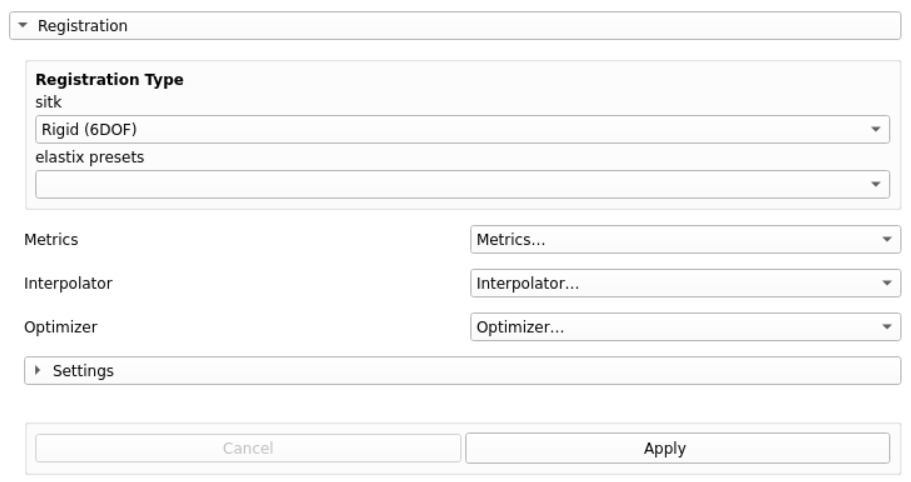
\includegraphics[width=0.5\textwidth]{images/registration_UI.png}
            \caption{Aperçu de l'UI de recalage.}
            \label{fig:registration_UI}
        \end{figure}

        \bigskip
        \subsubsubsection{Métriques}

        Ce sont des mesures de similarité statistiques qui partent du postulat qu'il existe un lien entre les intensités des deux images à recaler. L'extension en implémente quatre.

        \begin{itemize}
            \item \textbf{Mean Squares} Elle est utilisée pour minimiser la différence entre les intensités des voxels des images enregistrées.

            \item \textbf{Mattes Mutual Information} Elle utilise l'information mutuelle pour mesurer la similarité entre les images. L'information mutuelle mesure la quantité d'informations partagées entre deux images. La valeur liée à la métrique est \texttt{Number of Histogram Bins}, disponible sous l'onglet \textit{Settings}. Valeur par défaut~: 50.

            \item \textbf{Joint Histogram Mutual Information} Similaire à la métrique ci-dessus mais utilisant une méthode de calcul basée sur les histogrammes de Parzen. La valeur liée à cette métrique est \textit{Number of Histogram Bins}, disponible sous l'onglet \textit{Settings}. Valeur par défaut~: 20.

            \item \textbf{Correlation} Elle utilise le coefficient de corrélation de Pearson pour mesurer la similarité entre les images (mesure la corrélation entre les intensités des voxels des deux images).
        \end{itemize}

        \bigskip
        \subsubsubsection{Interpolateurs}

        Les interpolateurs (voir Figure~\ref{fig:registration_interpolator}) sont des fonctions d'image qui permettent de calculer les valeurs des voxels de l'image transformée à partir des valeurs des voxels de l'image originale. Quatre versions sont disponibles dans le module.

        \begin{itemize}
            \item \textbf{Linear} Interpolation linéaire.

            \item \textbf{Nearest Neighbor} Interpolation par la méthode des plus proches voisins. Cela consiste à attribuer à chaque point de la grille de destination la valeur du point le plus proche de la grille source.

            \item \textbf{B-Spline (1, 2, 3)} Interpolation via une fonction de base B-Spline, pour interpoler les valeurs des voxels de l'image transformée à partir des valeurs des voxels de l'image originale.

            \item \textbf{Gaussian} Interpolation via une fonction Gaussienne.
        \end{itemize}

        \bigskip

        \begin{figure}[!ht]
            \centering
            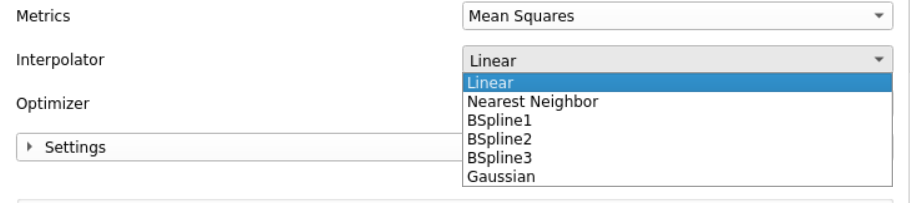
\includegraphics[width=0.5\textwidth]{images/registration_interpolator.png}
            \caption{Interpolateurs disponibles.}
            \label{fig:registration_interpolator}
        \end{figure}

        \bigskip
        \subsubsubsection{Optimiseurs}

        Ce sont des algorithmes qui permettent de trouver les paramètres optimaux pour une fonction de coût donnée. Ils sont utilisés pour trouver les paramètres de transformation qui minimisent la différence entre deux images.

        \begin{itemize}
            \item \textbf{Gradient Descent} Utilise le gradient de la métrique pour trouver le minimum local, voir la Figure~\ref{fig:registration_gd}. Les paramètres sont les suivants.

            \begin{itemize}
                \item \textit{Learning Rate} Paramètre qui contrôle la taille du pas de descente de gradient à chaque itération. Valeur par défaut~: 0.1

                \item \textit{Number of Iterations} Valeur par défaut~: 100.

                \item \textit{Convergence Minimum Value} Valeur qui indique à l'algorithme quand il doit s'arrêter. Valeur par défaut~: 1e-6.

                \item \textit{Convergence Window Size} Nombre d'itérations pour lesquelles l'algorithme doit converger avant d'arrêter. Valeur par défaut~: 10.
            \end{itemize}

            \item \textbf{Exhaustive}~: Méthode qui consiste à énumérer toutes les combinaisons possibles de paramètres pour trouver la meilleure solution. Les paramètres sont les suivants.

            \begin{itemize}
                \item \textit{Number of Steps} Nombre de pas pour chaque dimension de paramètre. Correspond aux paramètres d'une transformation Euler 3D. C'est un vecteur de 6 valeurs (angle x, y, z, translation x, y, z). Valeur par défaut~: 1, 1, 1, 0, 0, 0.

                \item \textit{Step Length} Longueur de pas pour chaque dimension de paramètre. Valeur par défaut~: $\pi$.

                \item \textit{Optimizer Scale} Permet de spécifier les échelles des paramètres dans l'optimiseur utilisé pour minimiser la fonction de coût. C'est un vecteur d'entier. Valeur par défaut~: 1, 1, 1, 1, 1, 1.
            \end{itemize}

            \item \textbf{LBFGSB}~: Algorithme d'optimisation quasi-Newtonien qui utilise une approximation de la matrice Hessienne pour trouver le minimum local. Il est plus robuste, plus rapide et efficace qu'une descente de gradient.

            \begin{itemize}
                \item \textit{Gradient Convergence Tolerance} Seuil pour laquelle l'algorithme considère que le gradient a convergé vers un minimum local. Valeur par défaut~: 1e-5.

                \item \textit{Number of Iterations} Valeur par défaut~: 100.

                \item \textit{Maximum Number of Corrections} Nombre maximum de corrections à appliquer avant d'arrêter l'algorithme. Une correction est une étape de mise à jour des paramètres de l'optimiseur. Valeur par défaut~: 5.

                \item \textit{Maximum Number of Function Evaluation} Valeur par défaut~: 1000.
            \end{itemize}
        \end{itemize}

        \bigskip

        \begin{figure}[!ht]
            \centering
            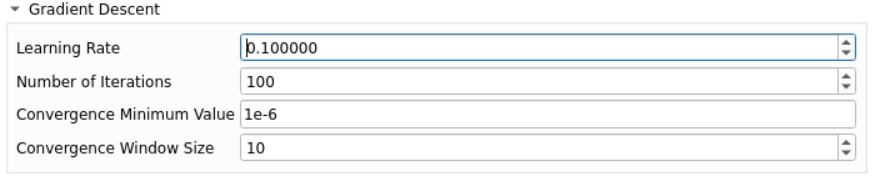
\includegraphics[width=0.5\textwidth]{images/registration_gd.png}
            \caption{Exemple des paramètres de la descente de gradient.}
            \label{fig:registration_gd}
        \end{figure}

        \bigskip
        \subsubsubsection{Recalage non-rigide}

        Les méthodes de recalages non rigides (B-Spline et Demons), ont des paramètres inhérent qui vont être détaillés ci-dessous.

        \begin{itemize}
            \item \textbf{B-Spline} Méthode de recalage déformable qui utilise des courbes B-Spline pour définir un champ de déformation continu qui fait correspondre chaque voxel d'une image en mouvement à un voxel correspondant dans une image fixe ou de référence. Ce recalage supporte une approche multi-résolution d'ordre 3 qui effectue d'abord l'enregistrement à une résolution inférieure avec moins de paramètres au premier niveau, puis adapte ou rééchantillonne les points de contrôle B-Spline à une résolution supérieure aux niveaux suivants. Voici les paramètres utilisés.

            \begin{itemize}
                \item \textit{Transform Domain Mesh Size} Nombre de points de contrôle utilisés pour définir la transformation B-Spline. Plus il est grand, plus le recalage sera précis mais long. Valeur par défaut~: 2.

                \item \textit{Scale Factor} Utilisé pour mettre à l'échelle la grille de points de contrôle B-Spline à chaque niveau de résolution. Valeur par défaut~: [1, 2, 4]. (Il ne peut pas être utilisé avec l'optimiseur LBFGSB, et devient inactif si sélectionné.)

                \item \textit{Shrink Factor} Utilisé pour déterminer la taille de l'image à chaque niveau de résolution. Valeur par défaut~: [4, 2, 1].

                \item \textit{Smoothing Sigmas} Utilisés pour lisser les images à chaque niveau de résolution. Valeur par défaut~: [2, 1, 0].
            \end{itemize}

            \item \textbf{Demons} Méthode de recalage non paramétrique qui estime le champ de déformation entre deux images en minimisant une fonction d'énergie qui mesure la différence entre les deux images. L'algorithme met à jour de manière itérative un champ de déformation qui fait correspondre une image à une autre jusqu'à convergence. Notre extension propose quatre variations de Demons. \textit{Original}, \textit{Diffeomorphic}, \textit{Symmetric Forces}, et \textit{Fast Symmetric Forces}. Voici leurs paramètres.

            \begin{itemize}
                \item \textit{Number of Iterations} Valeur par défaut~: 20.

                \item \textit{Standard Deviation} Utilisé pour contrôler l'ampleur du lissage appliqué au champ de déplacement. Valeur par défaut~: 1.
            \end{itemize}
        \end{itemize}

        \bigskip
        \subsubsubsection{Autres paramètres}

        Deux autres paramètres que l'on trouve dans les recalages non rigide, rigide et affines viennent compléter la gamme d'entrées du dictionnaire.

        \begin{itemize}
            \item \textit{Sampling Strategy} Spécifie comment les échantillons sont tirés du domaine d'image fixe pour calculer la valeur de la métrique. La stratégie \textit{None} utilise tous les voxels. \textit{Regular} échantillonne chaque n-ième voxel en parcourant l'image dans l'ordre des lignes de balayage. Et \textit{Random} échantillonne chaque n-ième voxel tout en parcourant l'image dans l'ordre de la ligne de balayage, puis dans chaque voxel, perturbé aléatoirement à partir du centre. Valeur par défaut~: \textit{Random}.

            \item \textit{Sampling Percentage} Définit le pourcentage de voxels échantillonnés pour l'évaluation métrique. Valeur par défaut~: 0.01.
        \end{itemize}

        \subsubsection{Limites}
        \label{subsubsec:limits-registration-implementation}

        La Figure~\ref{fig:registration_use_case} illustre à quoi ressemble l'interface utilisateur après sélection de quelques paramètres qui seront exportés dans le dictionnaire pour ensuite être utilisés dans le script \texttt{Rigid.py}. Sous cette forme minimal, l'interface utilisateur ne permet pas une maîtrise totale des algorithmes de recalage. Pour être exhaustif, beaucoup de paramètres auraient dû être rajoutés, mais dans un souci de clarté et de simplicité, seuls certains paramètres ont étés retenus. De plus, il faut être attentif aux paramètres lors d'un recalage non rigide avec B-Spline, en effet, si on utilise un \textit{Transform Domain Mesh Size} élevé avec un vecteur \textit{Scale Factor} conséquent, le recalage peut prendre énormément de temps. C'est à l'utilisateur d'ajuster chaque paramètre pour faire en sorte d'obtenir les résultats sous ses propres exigences (durée du recalage, précision). C'est pour cela que plusieurs options sont ouverts à l'utilisateur, selon ses besoins. Aussi, le recalage Demons nécessite d'avoir au préalable rééchantillonner l'image à recaler, il se peut que une erreur s'affiche, dans ce cas, il faut suivre les indications du message d'erreur. Enfin, il n'a pas toujours été possible de rediriger les sorties écrites vers le script principal. En l'état il affiche dans la console python les conditions d'arrêt uniquement pour les recalages rigide, B-Spline et affine. Le sortie écrite de Slicer Elastix n'a pas été implémenté, ni la sortie pour Demons qui n'utilise pas le même objet pour exécuter le recalage.

        \bigskip

        \begin{figure}[!ht]
            \centering
            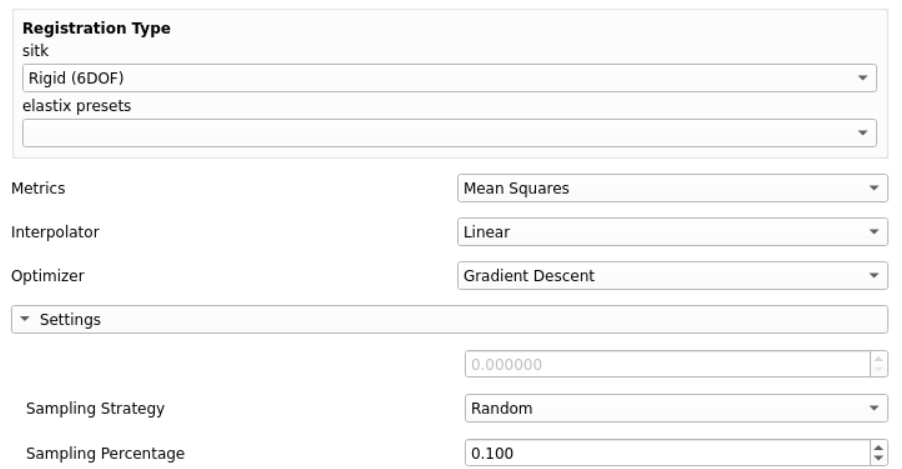
\includegraphics[width=0.5\textwidth]{images/registration_use_case.png}
            \caption{Cas utilisateur d'un recalage rigide avec divers paramètres sélectionnés.}
            \label{fig:registration_use_case}
        \end{figure}
    }

    % Calcul de carte de différence
    {
        \newpage
        \subsection{Carte de différence}
        \label{subsec:difference-map-implementation}

        La carte de différence a pour but d'évaluer l'erreur entre deux images. Elle apporte une estimation visuelle et permet d'évaluer les performances, avantages et désavantages des différents traitements et recalages effectués, en identifiant également les zones les plus impactées.

        Avec différentes techniques, il est possible de calculer une carte de différence en ayant en entrée deux images, dans notre cas l'image initiale et l'image recalée, puis d'améliorer sa visualisation.

        \bigskip

        Les bibliothèques \textit{VTK} et \textit{NumPy} ont été utilisées. Elles sont déjà présentes et utilisées dans 3D~Slicer. Les images sont stockées dans 3D~Slicer comme des volumes \textit{VTK}. Pour calculer la carte de différence efficacement, les deux images sont converties en tableaux \textit{NumPy}. \textit{NumPy} permet alors d'accéder à plusieurs fonctions optimisées.

        \bigskip

        Pour calculer une carte de différence via l'UI dédiée, il suffit de choisir un algorithme entre la valeur absolue de la différence et la différence de gradient, et éventuellement une taille de patch pour appliquer un filtre moyenneur et limiter ainsi le bruit.

        La carte de différence est calculée entre l'image d'entrée et l'image cible (sélectionnées préalablement dans l'interface supérieure). Une fois le calcul terminé, la carte de différence est affichée dans la vue dédiée, c'est-à-dire la vue jaune (en bas à gauche).

        \begin{figure}[!ht]
            \centering
            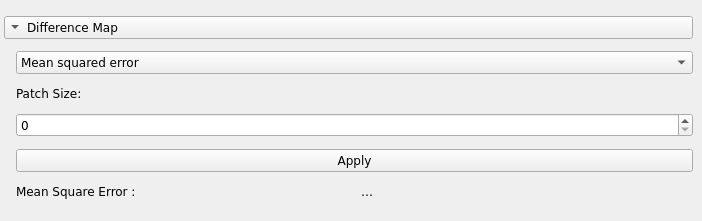
\includegraphics[width=0.5\textwidth]{images/UI_difference_map.png}
            \caption{Aperçu de l'UI de la carte de différence.}
            \label{fig:UI_difference_map}
        \end{figure}

        \subsubsection{Valeur absolue de la différence}
        \label{subsubsec:absolute-difference-difference-map-computation-implementation}

        Soient $A$ et $B$ respectivement les images d'entrée et cible sélectionnées, et $C$ la carte de différence. $C(i) = ||A(i) - B(i)||$, où $i$ est l'index d'un voxel dans $A$ et $B$.

        \bigskip

        L'avantage d'utiliser la valeur absolue dans le calcul de la carte de différence est qu'elle permet d'obtenir des résultats positifs qui reflètent l'amplitude de l'erreur de recalage. En effet, la valeur absolue ignore le signe des différences, ce qui permet de prendre en compte l'intensité des erreurs dans toutes les directions. Ainsi, si un voxel est mal aligné dans une certaine direction, la carte de différence va montrer une différence significative en termes d'amplitude, indépendamment de la direction de l'erreur.

        \begin{figure}[!ht]
            \centering
            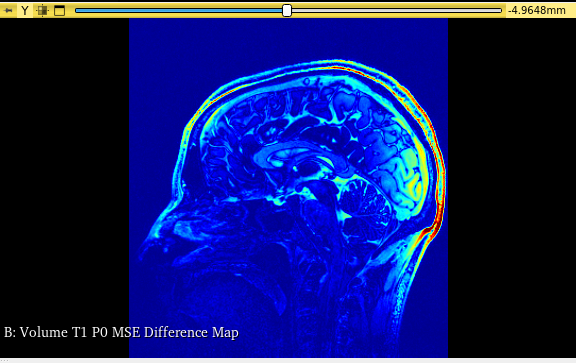
\includegraphics[width=0.5\textwidth]{images/absolute.png}
            \caption{Exemple de carte de différence en valeur absolue.}
            \label{fig:absolute}
        \end{figure}

        \subsubsection{Différence de gradient}
        \label{subsubsec:gradient-difference-difference-map-computation-implementation}

        Soient $A$ et $B$ respectivement les images d'entrée et cible sélectionnées, et $C$ la carte de différence. $C(v) = \nabla A(v) - \nabla B(v)$, où $\nabla A(v)$ et $\nabla B(v)$ sont les gradients de $A$ et $B$ respectivement, et $v$ est un voxel de $A$ et $B$. Le gradient de l'image est calculé grâce aux bibliothèques \textit{VTK} et \textit{NumPy}.

        \bigskip

        L'utilisation des gradients peut être pertinente car elle permet de quantifier la différence entre deux images en se basant sur les variations locales de l'intensité des voxels plutôt que sur leurs valeurs absolues. Cela peut être plus précis pour détecter les zones de l'image où le recalage a le plus d'impact, car les gradients mesurent les changements de l'intensité des voxels, ce qui est particulièrement pertinent pour les contours et les détails fins.

        \begin{figure}[!ht]
            \centering
            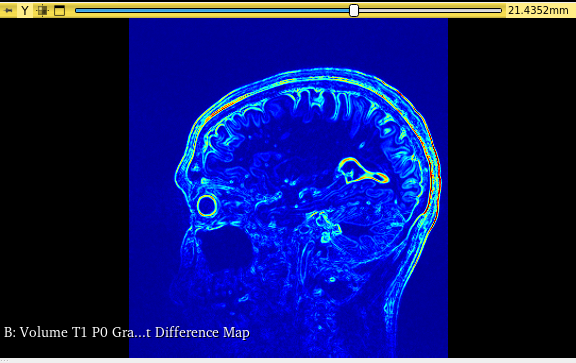
\includegraphics[width=0.5\textwidth]{images/gradient.png}
            \caption{Exemple de carte de différence de gradient.}
            \label{fig:gradient}
        \end{figure}

        \subsubsection{Filtre moyenneur avec noyau de convolution}
        \label{subsubsec:convolution-kernel-difference-map-computation-implementation}

        Ce filtre permet de flouter l'image et d'avoir une meilleur vue d'ensemble de la carte d'erreur et d'éliminer le bruit potentiel notamment sur la carte de différence de gradient. Il est applicable par l'utilisateur en entrant une taille de patch. Notre patch parcourt l'image pour moyenner la valeur du voxel et de ses voisins à l'aide de la bibliothèque \textit{SciPy} et sa méthode \texttt{convolve}.

        \begin{figure}[!ht]
            \centering
            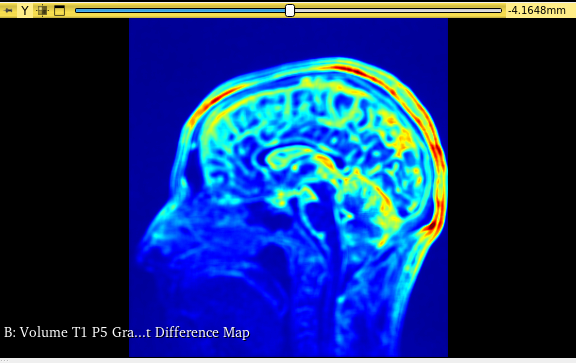
\includegraphics[width=0.5\textwidth]{images/convolve.png}
            \caption{Exemple d'un flou avec le filtre moyenneur ayant un patch de taille 5}
            \label{fig:convolve}
        \end{figure}

        \subsubsection{Look Up Table}
        \label{subsubsec:lut-difference-map-computation-implementation}

        La bibliothèque \textit{VTK} permet également d'appliquer une Look Up Table (LUT) pour améliorer la visualisation de la carte de différence. Cela permet de modifier la couleur de la carte de différence pour mettre en évidence certaines zones d'intérêt ou pour améliorer la lisibilité. Nous avons utilisé la LUT \textit{ColdToHotRainbow}, disponible dans 3D~Slicer.
    }

    % Plugins
    {
        \subsection{Plugins}
        \label{subsec:plugins}

        Les plugins sont un moyen simple, rapide et efficace d'ajouter de nouvelles fonctionnalités au module. Un plugin se caractérise par deux fichiers~: une interface graphique XML (\texttt{.ui}) et un script Python (\texttt{.py}).

        \bigskip

        L'interface graphique XML doit contenir tous les widgets que l'utilisateur veut manipuler pour paramétrer son algorithme. Le fichier \texttt{.ui} peut être rédigé manuellement ou plus simplement généré à l'aide d'outils dédiés tels que le concepteur prédéfini de 3D~Slicer ou Qt~Designer (inclus dans Qt~Creator).

        \bigskip

        Le script Python correspondant à l'algorithme, ou à un point d'entrée aux algorithmes souhaités dans le module d'extension. Il est donc tout à fait possible d'utiliser ce script pour intégrer un algorithme personnalisé en Python ou tout autre langage, voire même pour appeler directement des algorithmes de bibliothèques. Le script doit contenir une fonction \texttt{run}, qui reçoit quatre paramètres.

        \begin{itemize}
            \item \texttt{ui} Objet représentant l'interface graphique du plugin. Il permet d'accéder aux éléments de l'UI pour les modifier ou récupérer des paramètres. Ces éléments sont accessibles en utilisant \texttt{ui.findChild(type, name)}.

            \item \texttt{scene} Scène de 3D~Slicer (pour ajouter, supprimer ou modifier des volumes et d'autres nœuds).

            \item \texttt{input\_volume} Image d'entrée définie dans le module. Si aucun volume n'est sélectionné en entrée, sa valeur sera None.

            \item \texttt{target\_volume} Image cible définie dans le module. Si aucun volume n'est sélectionné en entrée, sa valeur sera None.
        \end{itemize}

        \bigskip

        Pour importer un plugin, une dernière section est présente dans le panneaux de traitement, \textit{Plugins}. Cette section est composée seulement d'un bouton \textit{Load Plugin} qui permet d'importer un plugin (Figure~\ref{fig:plugins-ui}).

        \begin{figure}[!ht]
            \centering
            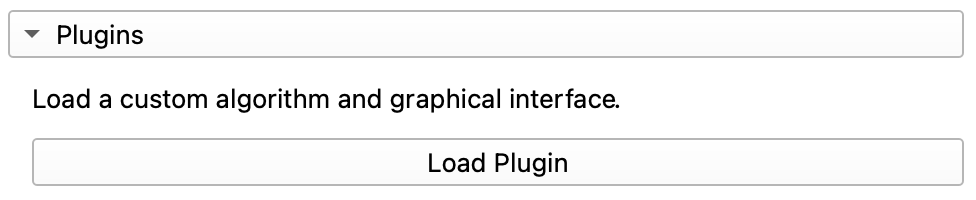
\includegraphics[width=0.5\textwidth]{images/plugins-ui.png}
            \caption{Aperçu de l'UI d'importation de plugins.}
            \label{fig:plugins-ui}
        \end{figure}

        Lors du clic sur le bouton, une fenêtre de dialogue apparaît contenant trois champs. Le champ du nom du plugin, ainsi que deux boutons pour charger une interface graphique XML et un script Python comme indiqué sur la Figure~\ref{fig:plugins-loading-ui}. Le clic sur chacun des deux boutons affiche respectivement une fenêtre de chargement de fichier limitée aux fichiers \texttt{.ui} et \texttt{.py}. Une fois un fichier choisi, son nom est affiché à gauche du bouton correspondant.

        \begin{figure}[!ht]
            \centering
            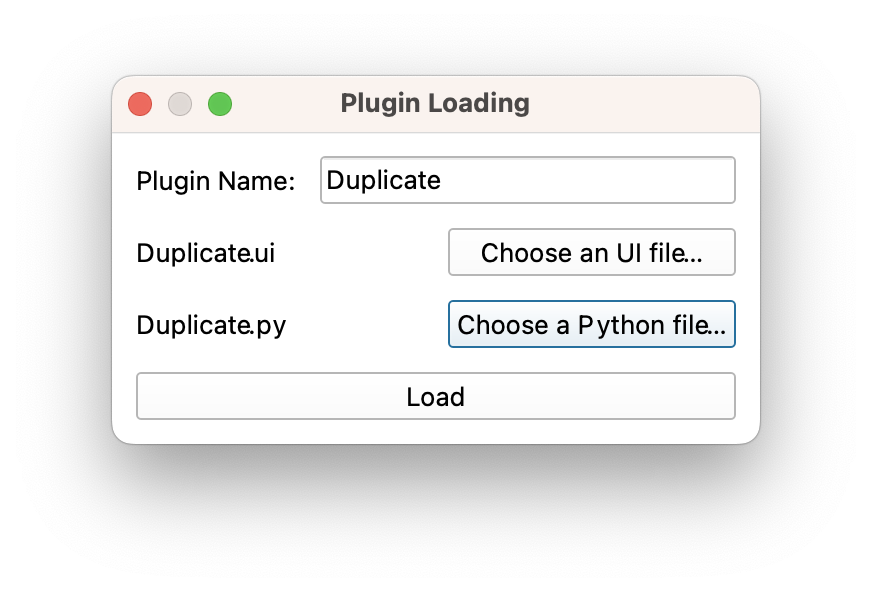
\includegraphics[width=0.75\textwidth]{images/plugin-loading-ui.png}
            \caption{Fenêtre de dialogue de chargement d'un plugin.}
            \label{fig:plugins-loading-ui}
        \end{figure}

        Enfin, lorsque le bouton \texttt{Load} est cliqué, la fenêtre de chargement de plugin se ferme. L'UI chargée est alors intégrée dans le panneau de traitements dans une sous-section dédiée définie par le nom du plugin, et un bouton \texttt{Run <Plugin Name>} est inséré afin de pouvoir faire appel au script chargé à tout moment. Cette intégration est représentée par la Figure~\ref{fig:plugins-integration-ui}.

        \begin{figure}[!ht]
            \centering
            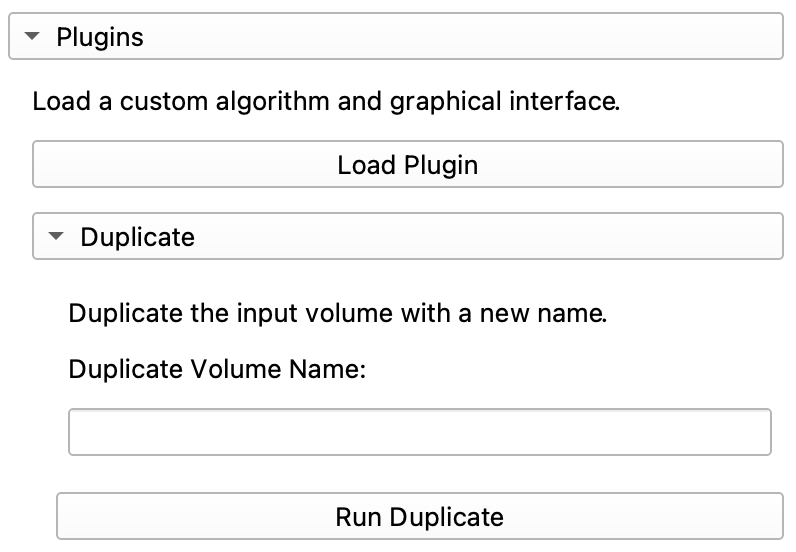
\includegraphics[width=0.5\textwidth]{images/plugins-integration-ui.png}
            \caption{Fenêtre de dialogue de chargement d'un plugin.}
            \label{fig:plugins-integration-ui}
        \end{figure}

        \bigskip

        L'importation de plugins est entièrement gérée par la méthode \texttt{Widget.setup\_plugin\_loading}. Cette méthode est très simple. Elle se charge d'initialiser le chargement de plugins une fois au démarrage par la méthode \texttt{Widget.setup} générale et c'est terminé, il n'y a plus besoin de recharger l'outil d'importation de plugins.

        Tout d'abord, un dictionnaire est défini représentant la liste de plugins, chaque nom étant associé au chemin d'accès du script Python. Celui de l'interface graphique XML n'est pas nécessaire car celle-ci est chargée directement lors de l'importation d'un plugin, alors que le script peut être appelé à tout moment lors de l'utilisation du module. Ensuite, le bouton de chargement de plugin est alors récupéré et lié à la sous-fonction d'importation décrite ci-après.

        \bigskip

        La sous-fonction d'importation \texttt{on\_plugin\_loading\_button\_clicked} se charge de créer la fenêtre de dialogue Qt permettant le chargement d'un plugin, représentée en Figure~\ref{fig:plugins-loading-ui}. Les boutons détaillés plus tôt sont donc liés à des actions spécifiques permettant d'ouvrir une fenêtre de chargement de fichier grâce à Qt (sous-fonctions spécifiques \texttt{on\_ui\_file\_button\_clicked} et \texttt{on\_python\_file\_button\_clicked}). Les chemins des fichiers ainsi récupérés sont gardés en mémoire temporairement. Le bouton de \textit{Load Plugin} est quant à lui lié à une autre sous fonction nommée \texttt{on\_load\_button\_clicked} et décrite ci-après.

        \bigskip

        Enfin, la sous-fonction \texttt{on\_load\_button\_clicked} permet quant elle de charger effectivement le plugin. Tout d'abord, le nom du plugin est vérifié car il ne peut y avoir plusieurs plugins de même nom, ainsi que la présence des fichiers requis. On peut alors charger l'UI depuis le fichier dédié grâce à la méthode de 3D~Slicer \texttt{util.loadUI}, en l'insérant dans une nouvelle section du panneau de traitements nommé en accord avec le plugin.

        On ajoute alors le bouton \texttt{Run <Plugin Name>} mentionné précédemment en le liant à l'appel de la fonction \texttt{run} du script Python qui lui est alors stocké dans le dictionnaire des plugins.
    }

    \newpage
}

% Conclusion
{
    \section{Conclusion}
    \label{sec:conclusion}

    Ce projet est achevé mais il existe de nombreuses possibilités d'améliorer cette proposition. Les User Stories ont toutes été traitées, nous offrons donc ici une solution efficace aux problèmes de dispersion et de complexité des différentes fonctionnalités implémentées dans 3D~Slicer concernant les prétraitements et le recalage, à laquelle s'ajoute une automatisation de certains traitements, une possibilité de comparaison via la carte de différence, et surtout l'ouverture vers le monde des possibles avec les plugins.

    % Bilan
    {
        \bigskip
        \subsection{Bilan}

        Tout d'abord, notre extension répond en effet aux critères d'acceptabilité de la \hyperref[us:registration]{US I} concernant les prétraitements. Conformément à la maquette mise en place (Figure~\ref{fig:ui-mock-up}), l'UI créée offre bien la possibilité de sélectionner une image à traiter et une image de référence grâce à des listes déroulantes (Figure~\ref{fig:input-target-ui}), et les affiche dans la disposition à droite, chacune dans une vue dédiée. De plus, notre extension comporte les trois prétraitements prévus et fonctionnels, à savoir la sélection de ROI par seuillage, le rognage manuel et automatique, ainsi que le rééchantillonnage. De manière similaire aux maquettes de paramétrage des prétraitements (Figures~\ref{fig:roi-ui-mock-up}, \ref{fig:cropping-ui-mock-up} et \ref{fig:resampling-ui-mock-up}), ceux-ci sont en effet paramétrables (Figures~\ref{fig:roi-selection-ui}, \ref{fig:manual-cropping-ui}, \ref{fig:automatic-cropping-ui}, et~\ref{fig:resampling-ui}). Finalement, lorsque pertinent, une prévisualisation du prétraitement à venir ou une visualisation finale peuvent s'afficher à la guise de l'utilisateur (Figures~\ref{fig:roi-selection-preview}, \ref{fig:roi-selection-view} et~\ref{fig:cropping-preview}).

        \bigskip

        Les critères d'acceptabilité concernant la \hyperref[us:registration]{US II} sur le recalage sont respectés, la section recalage est effective, fonctionnelle et a été testée minutieusement. Les utilisateurs finaux pourront recaler les images d'entrée et cible avec des paramètres Prédéfinis ou entrés par celui-ci, l'image recalée s'affichera dans la vue prévu à cet effet. En plus ce des critères, des ajouts bénéfiques et conviviaux pour les utilisateurs ne sont pas à négliger; l'activation du processus s'exécute en arrière plan, ainsi il n'est pas bloquant, en outre un bouton \textit{Cancel} est à la disposition de l'utilisateur si celui-ci trouve que le recalage prend trop de temps.

        \bigskip

        Enfin, la carte de différence répond à toutes les exigences, c'est-à-dire deux algorithmes différents permettant d'évaluer les endroits où le recalage a été le plus ou le moins efficace. La LUT vient appuyer sur les zones les plus impactées avec un gradient de couleur instinctif et l'opération noyau de convolution est efficace pour casser le bruit sur les cartes de gradient.

        \bigskip
    }

    % Perspectives
    {
        \bigskip
        \subsection{Perspectives}

        Au niveau des prétraitements, les perspectives d'améliorations sont nombreuses. Nous nous sommes effectivement concentrés sur des traitements généraux avec des paramètres minimaux. Mais tous ces prétraitements pourraient également posséder un mode "avancé" comprenant des paramètres plus spécifiques, ou simplement manuels, afin d'affiner l'utilisation selon les besoins. Ceci étant dit, il est tout de même possible de faire des traitements avancés en utilisant des plugins personnalisés.

        En particulier, la sélection de ROI pourrait être grandement améliorée avec une segmentation et non pas un seuillage binaire. L'utilisateur pourrait segmenter son image et alors choisir le(s) tissu(s) qu'il vise à sélectionner plus précisément.

        Concernant le rééchantillonnage, il pourrait être fait d'une manière supplémentaire, par exemple en rééchantillonnant les deux images sélectionnées vers une nouvelle résolution spatiale définie, autre que les deux déjà existantes. Ou encore, on pourrait également choisir un mode d'interpolation différent pour obtenir des voxels de valeurs différentes selon le cas. On rentre alors dans les paramétrisations avancées évoquées précédemment.

        \bigskip

        La prévisualisation de manière générale n'est pas encore optimisée. Que ce soit pour la sélection de ROI, le rognage manuel, ou le rognage automatique, le traitement est fait même si l'utilisateur ne le confirme jamais, afin de créer l'objet de prévisualisation. Une perspective d'optimisation viserait donc à créer l'objet de prévisualisation, sans avoir à effectuer le traitement dans tous les cas.

        De plus, concernant le rognage, on pourrait ajouter la possibilité d'interagir avec les points de contrôle, afin de permettre à l'utilisateur de définir encore plus précisément la zone à rogner.

        \bigskip

        Dans la partie dédiée au recalage le prochain jalon de développement aurait été la possibilité d'exécuter deux recalages sur une même image~: l'un à l'intérieur de la ROI et l'autre à l'extérieur, afin d'assurer lors du recalage une prise en compte des ROI.

        Notre extension pourrait également être améliorée pour permettre à l'utilisateur de comparer ses propres algorithmes de recalage en implémentant des métriques de performances entre les recalages en fonction de l'utilisation~: rapidité, précision, polyvalence.

        Enfin, on pourrait également se concentrer sur l'ajout d'autres bibliothèques de recalage plus spécifique aux images cérébrales comme BRAINS déjà disponible dans 3D~Slicer.

        \bigskip

        L'importation d'algorithmes via les plugins pourrait également être améliorée afin de faire tourner en arrière plan les scripts, à l'aide de l'extension \textit{Slicer Parallel Processing}.

        \bigskip

        La carte de différence aurait pu être amélioré de plusieurs façons. La première aurait été de mettre un chargement car l'opération du noyau de convolution peut prendre du temps, et par ailleurs paralléliser cette opération. Une autre aurait été de pouvoir choisir sa LUT, ça aurait augmenté l'accessibilité pour les personnes daltoniennes par exemple. Enfin devoir appuyer sur le bouton \textit{Apply} à chaque modification peut casser l'ergonomie, une carte de différence automatique aurait pu être mieux mais demande une meilleur gestion de la mémoire.
    }

    % Notes de fin
    {
        \bigskip
        \subsection{Notes de fin}

        La fin des réunions s'est conclue sur une satisfaction des deux parties, le client satisfait par la solution, et nous, développeurs sommes satisfaits et fiers d'avoir mené un projet qui sera utilisé voire amélioré. Nous avons apporté notre pierre à l'édifice qu'est 3D~Slicer, et nous sommes convaincus que notre développement extensible sera reconnu comme pratique pour laisser place à de nombreuses évolutions.
    }

    \newpage
}

% Références
{
    \bibliography{references}

    \newpage
}

% Annexes
{
    \section{Annexes}
    \label{sec:annexes}

    \begin{figure}[!ht]
        \centering
        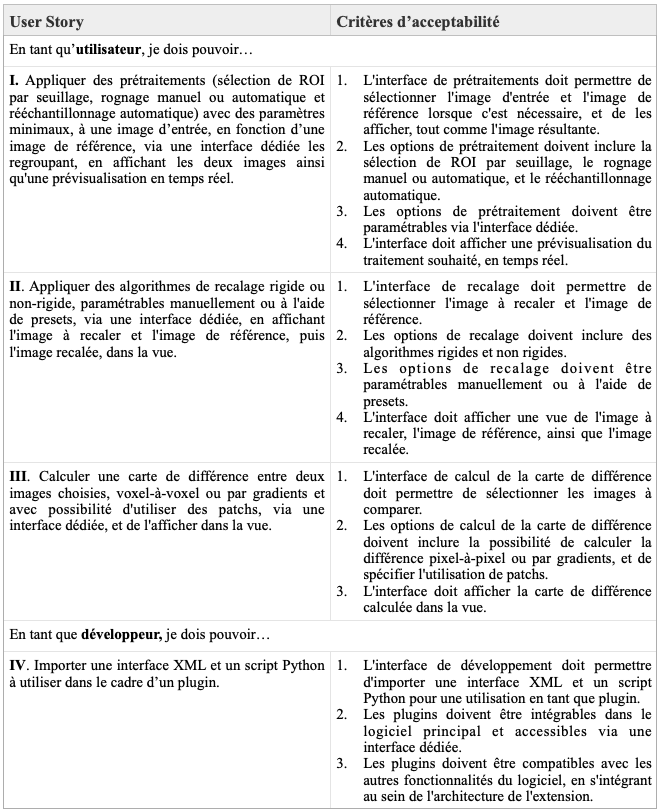
\includegraphics[height=0.7\textheight]{images/us-recap.png}
        \caption{Tableau récapitulatif des User Stories et leurs critères d'acceptabilité respectifs.}
        \label{fig:us-recap}
    \end{figure}
}

\end{document}
